%%%%%%%%%%%%%%%%%%%%%%%%%%%%%%%%%%%%%%%%%%%%%%%%%%%%%%%%%%
%%%%%%%%%%%%%%%%%%%%%%%%%%%%%%%%%%%%%%%%%%%%%%%%%%%%%%%%%%
\subsection{Introduction}
%%%%%%%%%%%%%%%%%%%%%%%%%%%%%%%%%%%%%%%%%%%%%%%%%%%%%%%%%%
%%%%%%%%%%%%%%%%%%%%%%%%%%%%%%%%%%%%%%%%%%%%%%%%%%%%%%%%%%

%%%%%%%%%%%%%%%%%%%%%%%%%%%%%%%%%%%%%%%%%%%%%%%%%%%%%%%%%%
\frame {\frametitle{Introduction}
%%%%%%%%%%%%%%%%%%%%%%%%%%%%%%%%%%%%%%%%%%%%%%%%%%%%%%%%%%
  \begin{itemize}
  \item \textbf{Collection and analysis of enormous datasets is at the heart
    of innovation in many organizations}
    \begin{itemize}
    \item E.g.: web crawls, search logs, click streams
    \end{itemize}

    \vspace{20pt}

  \item \textbf{Manual inspection before batch processing}
    \begin{itemize}
    \item Very often engineers look for exploitable trends in their
      data to drive the design of more sophisticated techniques
    \item This is difficult to do in practice, given the sheer size of
      the datasets
    \end{itemize}

    \vspace{20pt}

  \item \textbf{The MapReduce model has its own limitations}
    \begin{itemize}
    \item One input
    \item Two-stage, two operators
    \item Rigid data-flow
    \end{itemize}
  \end{itemize}
}

%%%%%%%%%%%%%%%%%%%%%%%%%%%%%%%%%%%%%%%%%%%%%%%%%%%%%%%%%%
\frame {\frametitle{MapReduce limitations}
%%%%%%%%%%%%%%%%%%%%%%%%%%%%%%%%%%%%%%%%%%%%%%%%%%%%%%%%%%
  \begin{itemize}
  \item \textbf{Very often tricky workarounds are
      required}\footnote{The term workaround should not only be
      intended as negative.}
    \begin{itemize}
    \item This is very often exemplified by the difficulty in
      performing \texttt{JOIN} operations
    \end{itemize}
    
    \vspace{20pt}
    
  \item \textbf{Custom code required even for basic operations}
    \begin{itemize}
    \item Projection and Filtering need to be ``rewritten'' for each job
    \end{itemize}
    
    \vspace{20pt}
    
  \item[$\to$] Code is difficult to reuse and maintain
  \item[$\to$] Semantics of the analysis task are obscured
  \item[$\to$] Optimizations are difficult due to opacity of
    \texttt{Map} and \texttt{Reduce} 

  \end{itemize} 
}

%%%%%%%%%%%%%%%%%%%%%%%%%%%%%%%%%%%%%%%%%%%%%%%%%%%%%%%%%%
%%%%%%%%%%%%%%%%%%%%%%%%%%%%%%%%%%%%%%%%%%%%%%%%%%%%%%%%%%
\subsubsection{Use Cases}
%%%%%%%%%%%%%%%%%%%%%%%%%%%%%%%%%%%%%%%%%%%%%%%%%%%%%%%%%%
%%%%%%%%%%%%%%%%%%%%%%%%%%%%%%%%%%%%%%%%%%%%%%%%%%%%%%%%%%
\frame {\frametitle{Use Cases}
%%%%%%%%%%%%%%%%%%%%%%%%%%%%%%%%%%%%%%%%%%%%%%%%%%%%%%%%%%
  \begin{beamerboxesrounded}{}
	\begin{center}
          \textbf{Rollup aggregates}
	\end{center}    
  \end{beamerboxesrounded}

  \begin{itemize}
  \item \textbf{Compute aggregates against user activity logs, web
      crawls, etc.}
    \begin{itemize}
    \item Example: compute the frequency of search terms aggregated
      over days, weeks, month
    \item Example: compute frequency of search terms aggregated over
      geographical location, based on IP addresses
    \end{itemize}

    \vspace{10pt}

  \item \textbf{Requirements} 
    \begin{itemize}
    \item Successive aggregations
    \item Joins followed by aggregations
    \end{itemize}

    \vspace{10pt}

  \item \textbf{Pig vs. OLAP systems}
    \begin{itemize}
    \item Datasets are too big
    \item \textbf{Data curation} is too costly
    \end{itemize}
  \end{itemize}
}

%%%%%%%%%%%%%%%%%%%%%%%%%%%%%%%%%%%%%%%%%%%%%%%%%%%%%%%%%%
\frame {\frametitle{Use Cases}
%%%%%%%%%%%%%%%%%%%%%%%%%%%%%%%%%%%%%%%%%%%%%%%%%%%%%%%%%%
 \begin{beamerboxesrounded}{}
	\begin{center}
          \textbf{Temporal Analysis}
	\end{center}    
  \end{beamerboxesrounded}

  \begin{itemize}
  \item \textbf{Study how search query distributions change over time}
    \begin{itemize}
    \item Correlation of search queries from two distinct time periods (groups)
    \item Custom processing of the queries in each correlation group
    \end{itemize}

    \vspace{20pt}

  \item \textbf{Pig supports operators that minimize memory footprint}
    \begin{itemize}
    \item Instead, in a RDBMS such operations typically involve
      \texttt{JOINS} over very large datasets that do not fit in
      memory and thus become slow
    \end{itemize}

  \end{itemize}
}

%%%%%%%%%%%%%%%%%%%%%%%%%%%%%%%%%%%%%%%%%%%%%%%%%%%%%%%%%%
\frame {\frametitle{Use Cases}
%%%%%%%%%%%%%%%%%%%%%%%%%%%%%%%%%%%%%%%%%%%%%%%%%%%%%%%%%%
 \begin{beamerboxesrounded}{}
	\begin{center}
          \textbf{Session Analysis}
	\end{center}    
  \end{beamerboxesrounded}

  \begin{itemize}
  \item \textbf{Study sequences of page views and clicks}
  
    \vspace{20pt}
  
  \item \textbf{Example of typical aggregates}
    \begin{itemize}
    \item Average length of user session
    \item Number of links clicked by a user before leaving a website
    \item Click pattern variations in time
    \end{itemize}
  
    \vspace{20pt}
  
  \item \textbf{Pig supports advanced data structures, and UDFs}
    
  \end{itemize}
}

%%%%%%%%%%%%%%%%%%%%%%%%%%%%%%%%%%%%%%%%%%%%%%%%%%%%%%%%%%
%%%%%%%%%%%%%%%%%%%%%%%%%%%%%%%%%%%%%%%%%%%%%%%%%%%%%%%%%%
\subsection{Overview}
%%%%%%%%%%%%%%%%%%%%%%%%%%%%%%%%%%%%%%%%%%%%%%%%%%%%%%%%%%
%%%%%%%%%%%%%%%%%%%%%%%%%%%%%%%%%%%%%%%%%%%%%%%%%%%%%%%%%%

%%%%%%%%%%%%%%%%%%%%%%%%%%%%%%%%%%%%%%%%%%%%%%%%%%%%%%%%%%
\frame {\frametitle{Pig Latin}
%%%%%%%%%%%%%%%%%%%%%%%%%%%%%%%%%%%%%%%%%%%%%%%%%%%%%%%%%%
  \begin{itemize}
  \item \textbf{Pig Latin, a high-level programming language initially developed at Yahoo!, now at HortonWorks}
    \begin{itemize}
    \item Combines the best of both declarative and imperative worlds
      \begin{itemize}
      \item High-level declarative querying in the spirit of SQL
      \item Low-level, procedural programming \'a la MapReduce
      \end{itemize}
    \end{itemize}

    \vspace{20pt}

  \item \textbf{Pig Latin features}
    \begin{itemize}
    \item Multi-valued, nested data structures instead of flat tables
    \item Powerful data transformations primitives, including joins
    \end{itemize}

    \vspace{20pt}

  \item \textbf{Pig Latin program}
    \begin{itemize}
    \item Made up of a series of operations (or transformations)
    \item Each operation is applied to input data and produce output
      data
    \item[$\to$] A Pig Latin program describes a data flow
    \end{itemize}

  \end{itemize}
}

%%%%%%%%%%%%%%%%%%%%%%%%%%%%%%%%%%%%%%%%%%%%%%%%%%%%%%%%%%
\frame {\frametitle{Example 1}
%%%%%%%%%%%%%%%%%%%%%%%%%%%%%%%%%%%%%%%%%%%%%%%%%%%%%%%%%%
  \begin{beamerboxesrounded}{}
	\begin{center}
          \textbf{Pig Latin premiere}
	\end{center}    
  \end{beamerboxesrounded}

  
  \begin{itemize}
  \item \textbf{Assume we have the following table:}
  \end{itemize}

  \vspace{10pt}

  \texttt{urls: (url, category, pagerank)}

  \begin{itemize}
  \item Where:
    \begin{itemize}
    \item \texttt{url}: is the url of a web page
    \item \texttt{category}: corresponds to a pre-defined category for
      the web page
    \item \texttt{pagerank}: is the numerical value of the pagerank
      associated to a web page
    \end{itemize}
  \end{itemize}

  \begin{itemize}
  \item[$\to$] \textit{Find, for each sufficiently large category, the
    average page rank of high-pagerank urls in that category}
  \end{itemize}
}

%%%%%%%%%%%%%%%%%%%%%%%%%%%%%%%%%%%%%%%%%%%%%%%%%%%%%%%%%%
\frame {\frametitle{Example 1}
%%%%%%%%%%%%%%%%%%%%%%%%%%%%%%%%%%%%%%%%%%%%%%%%%%%%%%%%%%
  \begin{beamerboxesrounded}{}
	\begin{center}
          \textbf{SQL}
	\end{center}    
  \end{beamerboxesrounded}

\vspace{60pt}


    \noindent \texttt{SELECT category, AVG(pagerank) }\\
    \texttt{FROM urls WHERE pagerank > 0.2 }\\
    \texttt{GROUP BY category HAVING COUNT(*) > $10^6$}
  
  
}

%%%%%%%%%%%%%%%%%%%%%%%%%%%%%%%%%%%%%%%%%%%%%%%%%%%%%%%%%%
\frame {\frametitle{Example 1}
%%%%%%%%%%%%%%%%%%%%%%%%%%%%%%%%%%%%%%%%%%%%%%%%%%%%%%%%%%
  \begin{beamerboxesrounded}{}
	\begin{center}
          \textbf{Pig Latin}
	\end{center}    
  \end{beamerboxesrounded}


\vspace{60pt}

\begin{footnotesize}

  \noindent \texttt{good\_urls = FILTER urls BY pagerank > 0.2;}\\
    \texttt{groups = GROUP good\_urls BY category;}\\
    \texttt{big\_groups = FILTER groups BY COUNT(good\_urls) > $10^6$;}\\
    \texttt{output = FOREACH big\_groups GENERATE}\\
    \texttt{category, AVG(good\_urls.pagerank);}

\end{footnotesize}
}

%%%%%%%%%%%%%%%%%%%%%%%%%%%%%%%%%%%%%%%%%%%%%%%%%%%%%%%%%%
\frame {\frametitle{Example 2}
%%%%%%%%%%%%%%%%%%%%%%%%%%%%%%%%%%%%%%%%%%%%%%%%%%%%%%%%%%
\begin{itemize}
  \item User data in one file, website data in another
  \item Find the top 5 most visited sites
  \item Group by users aged in the range (18,25)
\end{itemize}

\begin{figure}[h]
  \centering
  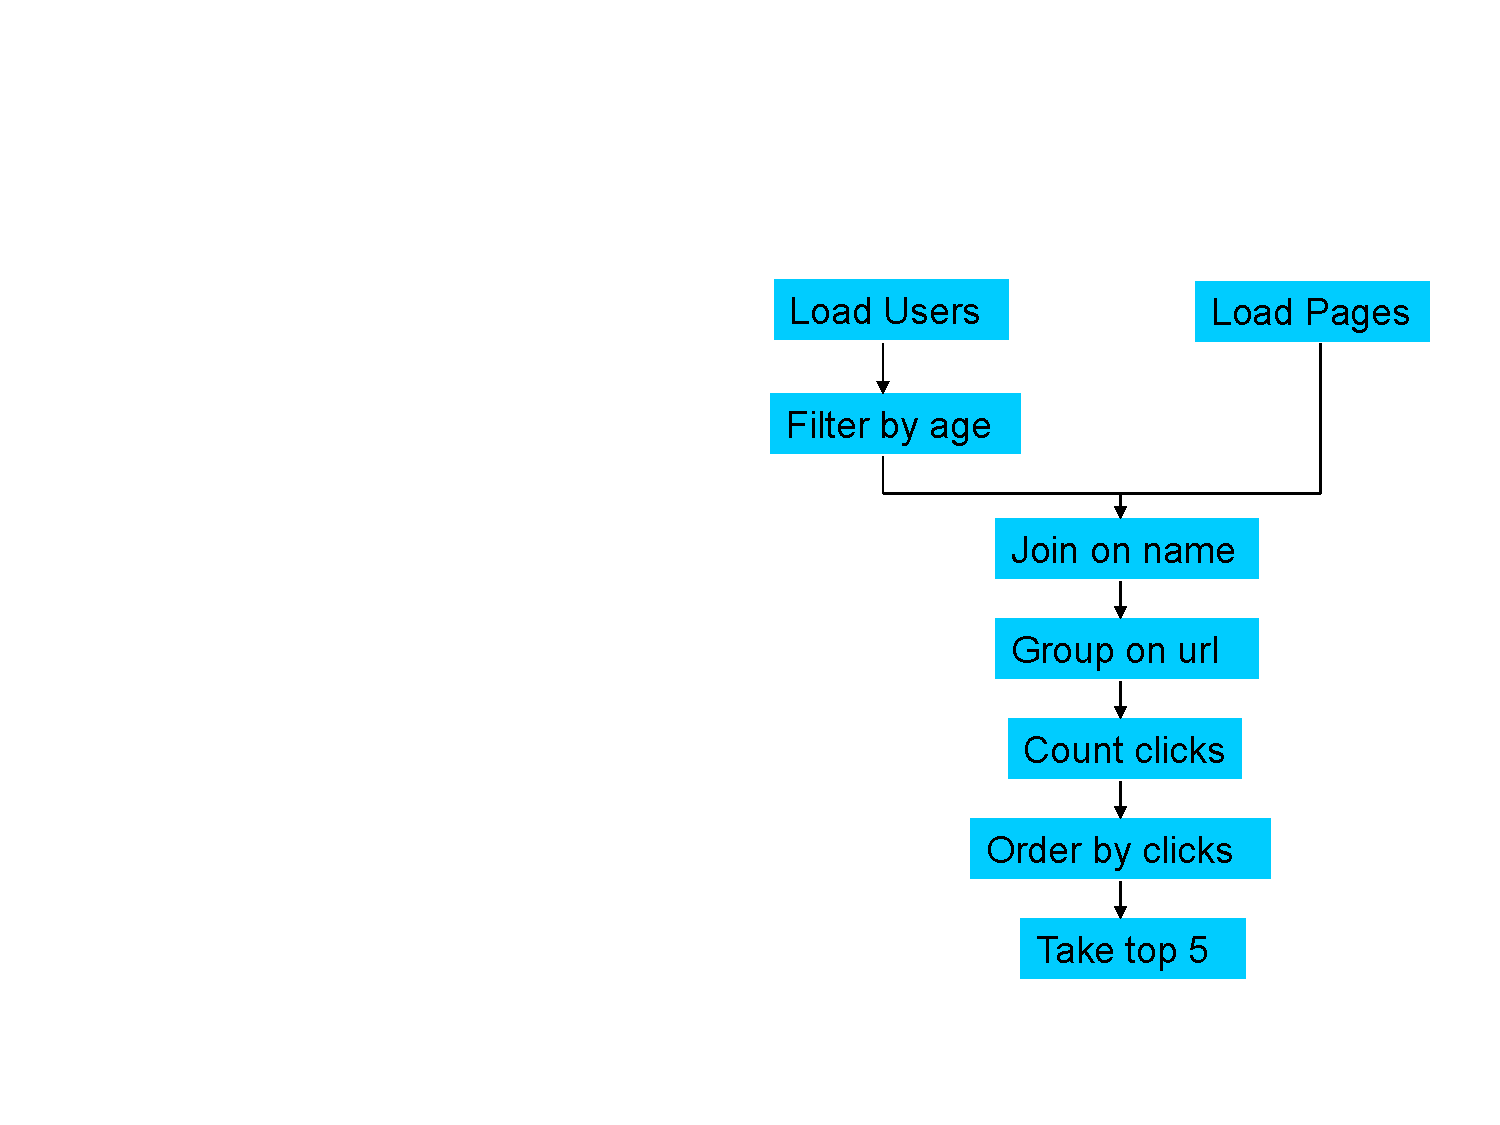
\includegraphics[scale=0.5]{./Figures/example2_plan}
\end{figure}
}

%%%%%%%%%%%%%%%%%%%%%%%%%%%%%%%%%%%%%%%%%%%%%%%%%%%%%%%%%%
\frame {\frametitle{Example 2: in MapReduce}
%%%%%%%%%%%%%%%%%%%%%%%%%%%%%%%%%%%%%%%%%%%%%%%%%%%%%%%%%%

\begin{figure}[h]
  \centering
  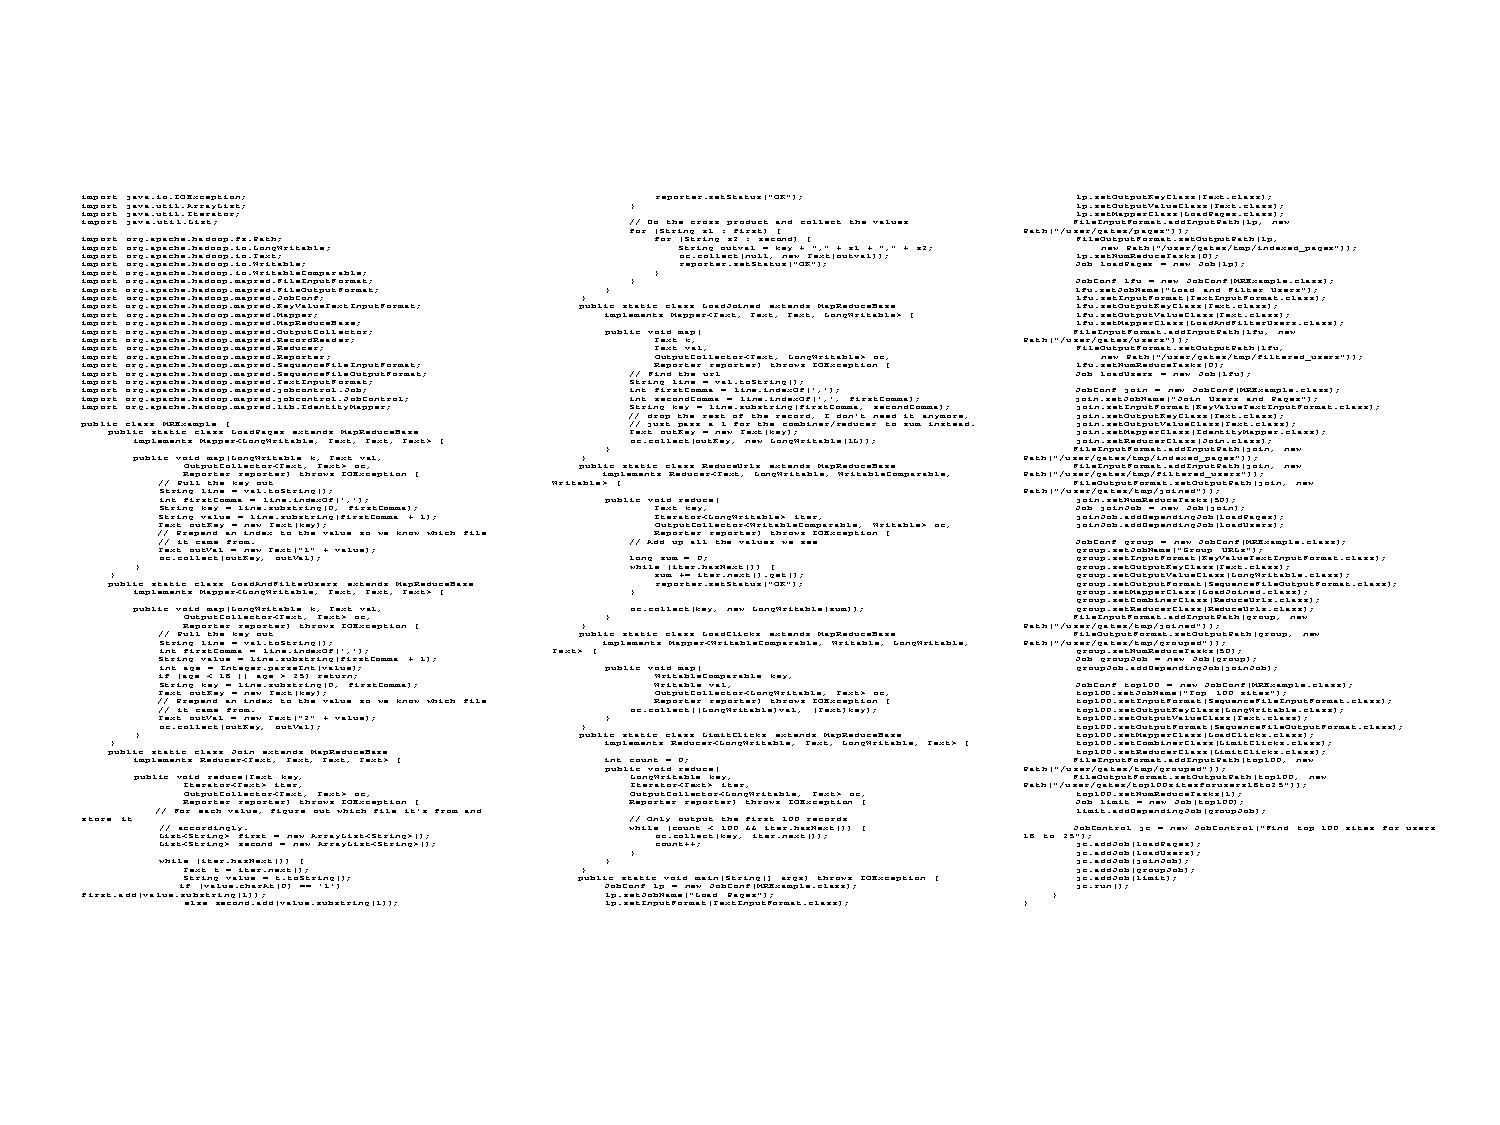
\includegraphics[scale=0.5]{./Figures/example2_mr}
\end{figure}

\begin{itemize}
  \item Hundreds lines of code; hours to write
\end{itemize}

}

%%%%%%%%%%%%%%%%%%%%%%%%%%%%%%%%%%%%%%%%%%%%%%%%%%%%%%%%%%
\frame {\frametitle{Example 2: in Pig}
%%%%%%%%%%%%%%%%%%%%%%%%%%%%%%%%%%%%%%%%%%%%%%%%%%%%%%%%%%
\begin{footnotesize}

\noindent \texttt{Users = load 'users' as (name, age);} \\
\texttt{Fltrd = filter Users by age >= 18 and age <= 25;} \\
\texttt{Pages = load 'pages' as (user, url);} \\
\texttt{Jnd = join Fltrd by name, Pages by user; Grpd = group Jnd by url;} \\
\texttt{Smmd = foreach Grpd generate group, COUNT(Jnd) as clicks;} \\
\texttt{Srtd = order Smmd by clicks desc; Top5 = limit Srtd 5;} \\
\texttt{store Top5 into 'top5sites';}
\end{footnotesize}

\begin{itemize}
  \item Few lines of code; few minutes to write
\end{itemize}

}

\frame {\frametitle{Pig Execution environment}
  \begin{itemize}
  \item \textbf{How do we go from Pig Latin to MapReduce?}
    \begin{itemize}
    \item The Pig system is in charge of this
    \item Complex execution environment that interacts with Hadoop
      MapReduce
    \item[$\to$] The programmer focuses on the data and analysis
    \end{itemize}

    \vspace{20pt}

  \item \textbf{Pig Compiler}
    \begin{itemize}
    \item Pig Latin operators are translated into MapReduce code
    \item {\color{red}NOTE}: in some cases, hand-written MapReduce
      code performs better
    \end{itemize}

    \vspace{20pt}

  \item \textbf{Pig Optimizer}\footnote{Currently, rule-based optimization only.}
    \begin{itemize}
    \item Pig Latin data flows undergo an (automatic) optimization phase\footnote{Optimizations can be selectively disabled.}
    \item These optimizations are borrowed from the RDBMS community
    \end{itemize}
    
  \end{itemize}
}

%%%%%%%%%%%%%%%%%%%%%%%%%%%%%%%%%%%%%%%%%%%%%%%%%%%%%%%%%%
%%%%%%%%%%%%%%%%%%%%%%%%%%%%%%%%%%%%%%%%%%%%%%%%%%%%%%%%%%
\subsubsection{Comparison with RDBMS}
%%%%%%%%%%%%%%%%%%%%%%%%%%%%%%%%%%%%%%%%%%%%%%%%%%%%%%%%%%
%%%%%%%%%%%%%%%%%%%%%%%%%%%%%%%%%%%%%%%%%%%%%%%%%%%%%%%%%%

%%%%%%%%%%%%%%%%%%%%%%%%%%%%%%%%%%%%%%%%%%%%%%%%%%%%%%%%%%
\frame {\frametitle{Pig and Pig Latin}
%%%%%%%%%%%%%%%%%%%%%%%%%%%%%%%%%%%%%%%%%%%%%%%%%%%%%%%%%%
  \begin{itemize}
  \item \textbf{Pig is not a RDBMS!}
    \begin{itemize}
    \item This means it is not suitable for all data processing tasks
    \end{itemize}

    \vspace{20pt}

  \item \textbf{Designed for batch processing}
    \begin{itemize}
    \item Of course, since it compiles to MapReduce
    \item Of course, since data is materialized as files on HDFS
    \end{itemize}

    \vspace{20pt}

  \item \textbf{{\color{red}NOT} designed for random access}
    \begin{itemize}
    \item Query selectivity does not match that of a RDBMS
    \item Full-scans oriented!
    \end{itemize}

  \end{itemize}
}

%%%%%%%%%%%%%%%%%%%%%%%%%%%%%%%%%%%%%%%%%%%%%%%%%%%%%%%%%%
\frame {\frametitle{Comparison with RDBMS}
%%%%%%%%%%%%%%%%%%%%%%%%%%%%%%%%%%%%%%%%%%%%%%%%%%%%%%%%%%
  \begin{itemize}
  \item \textbf{It may seem that Pig Latin is similar to SQL}
    \begin{itemize}
    \item We'll see several examples, operators, etc. that resemble
      SQL statements
    \end{itemize}

    \vspace{20pt}

  \item \textbf{Data-flow vs. declarative programming language}
    \begin{itemize}
    \item Data-flow:
      \begin{itemize}
      \item Step-by-step set of operations
      \item Each operation is a {\color{red}single transformation}
      \end{itemize}
    \item Declarative:
      \begin{itemize}
      \item Set of constraints
      \item Applied together to an input to generate output
      \end{itemize}
    \end{itemize}

    \vspace{20pt}

  \item[$\to$] \textbf{With Pig Latin it's like working at the query planner}

  \end{itemize}
}

%%%%%%%%%%%%%%%%%%%%%%%%%%%%%%%%%%%%%%%%%%%%%%%%%%%%%%%%%%
\frame {\frametitle{Comparison with RDBMS}
%%%%%%%%%%%%%%%%%%%%%%%%%%%%%%%%%%%%%%%%%%%%%%%%%%%%%%%%%%
  \begin{itemize}
  \item \textbf{RDBMS store data in tables}
    \begin{itemize}
    \item Schema are predefined and strict
    \item Tables are flat
    \end{itemize}

    \vspace{20pt}

  \item \textbf{Pig and Pig Latin work on more complex data structures}
    \begin{itemize}
    \item Schema can be defined at run-time for readability
    \item \textit{Pigs eat anything!}
    \item UDF and streaming together with nested data structures make
      Pig and Pig Latin more flexible
    \end{itemize}


  \end{itemize}

}







%%%%%%%%%%%%%%%%%%%%%%%%%%%%%%%%%%%%%%%%%%%%%%%%%%%%%%%%%%
%%%%%%%%%%%%%%%%%%%%%%%%%%%%%%%%%%%%%%%%%%%%%%%%%%%%%%%%%%
\subsection{Features and Motivations}
%%%%%%%%%%%%%%%%%%%%%%%%%%%%%%%%%%%%%%%%%%%%%%%%%%%%%%%%%%
%%%%%%%%%%%%%%%%%%%%%%%%%%%%%%%%%%%%%%%%%%%%%%%%%%%%%%%%%%


%%%%%%%%%%%%%%%%%%%%%%%%%%%%%%%%%%%%%%%%%%%%%%%%%%%%%%%%%%
\frame {\frametitle{Dataflow Language}
%%%%%%%%%%%%%%%%%%%%%%%%%%%%%%%%%%%%%%%%%%%%%%%%%%%%%%%%%%
  \begin{itemize}
  \item \textbf{A Pig Latin program specifies a series of steps}
    \begin{itemize}
    \item Each step is a {\color{red}single}, high level data transformation
    \item Stylistically different from SQL
    \end{itemize}

    \vspace{20pt}

  \item \textbf{With reference to Example 1}
    \begin{itemize}
    \item The programmer supply an order in which each operation will be done
    \end{itemize}

    \vspace{20pt}

  \item \textbf{Consider the following snippet}
  \end{itemize}


\noindent \texttt{spam\_urls = FILTER urls BY isSpam(url);\\
culprit\_urls = FILTER spam\_urls BY pagerank > 0.8;}
}

%%%%%%%%%%%%%%%%%%%%%%%%%%%%%%%%%%%%%%%%%%%%%%%%%%%%%%%%%%
\frame {\frametitle{Dataflow Language}
%%%%%%%%%%%%%%%%%%%%%%%%%%%%%%%%%%%%%%%%%%%%%%%%%%%%%%%%%%
  \begin{itemize}
  \item \textbf{Data flow optimizations}
    \begin{itemize}
    \item Explicit sequences of operations can be overridden
    \item Use of high-level, relational-algebra-style primitives
      (\texttt{GROUP}, \texttt{FILTER},...) allows using traditional
      RDBMS optimization techniques
    \end{itemize}

    \vspace{20pt}

  \item[$\to$] \textbf{NOTE: it is necessary to check whether such
    optimizations are beneficial or not, by hand}

    \vspace{20pt}

  \item \textbf{Pig Latin allows Pig to perform optimizations that would
    otherwise by a tedious manual exercise if done at the MapReduce
    level
}
  \end{itemize}
}


%%%%%%%%%%%%%%%%%%%%%%%%%%%%%%%%%%%%%%%%%%%%%%%%%%%%%%%%%%
\frame {\frametitle{Quick Start and Interoperability}
%%%%%%%%%%%%%%%%%%%%%%%%%%%%%%%%%%%%%%%%%%%%%%%%%%%%%%%%%%
  \begin{itemize}
  \item \textbf{Data I/O is greatly simplified in Pig}
    \begin{itemize}
    \item No need to curate, bulk import, parse, apply schema, create
      indexes that traditional RDBMS require
    \item Standard and ad-hoc ``readers'' and ``writers'' facilitate
      the task of ingesting and producing data in arbitrary formats
    \end{itemize}

    \vspace{20pt}

  \item \textbf{Pig can work with a wide range of other tools}

    \vspace{20pt}

  \item \textbf{Why RDBMS have stringent requirements?}
    \begin{itemize}
    \item To enable transactional consistency guarantees
    \item To enable efficient point lookup (using physical indexes)
    \item To enable data curation on behalf of the user
    \item To enable other users figuring out what the data is, by
      studying the schema
    \end{itemize}
  \end{itemize}
}

%%%%%%%%%%%%%%%%%%%%%%%%%%%%%%%%%%%%%%%%%%%%%%%%%%%%%%%%%%
\frame {\frametitle{Quick Start and Interoperability}
%%%%%%%%%%%%%%%%%%%%%%%%%%%%%%%%%%%%%%%%%%%%%%%%%%%%%%%%%%
  \begin{itemize}
  \item \textbf{Why is Pig so flexible?}
    \begin{itemize}
    \item Supports {\color{red}read-only workloads}
    \item Supports {\color{red}scan-only workloads} (no lookups)
    \item[$\to$] No need for transactions nor indexes
    \end{itemize}

    \vspace{20pt}

  \item \textbf{Why data curation is not required?}
    \begin{itemize}
    \item Very often, Pig is used for ad-hoc data analysis
    \item Work on temporary datasets, then throw them out!
    \item[$\to$] Curation is an overkill
    \end{itemize}

    \vspace{20pt}

  \item \textbf{Schemas are optional}
    \begin{itemize}
    \item Can apply one on the fly, at runtime
    \item Can refer to fields using positional notation
    \item E.g.: \texttt{good\_urls = FILTER urls BY \$2 > 0.2}
    \end{itemize}
  \end{itemize}
}

%%%%%%%%%%%%%%%%%%%%%%%%%%%%%%%%%%%%%%%%%%%%%%%%%%%%%%%%%%
\frame {\frametitle{Nested Data Model}
%%%%%%%%%%%%%%%%%%%%%%%%%%%%%%%%%%%%%%%%%%%%%%%%%%%%%%%%%%
  \begin{itemize}
  \item \textbf{Easier for ``programmers'' to think of nested data
      structures}
    \begin{itemize}
    \item E.g.: capture information about positional occurrences of
      terms in a collection of documents
    \item \texttt{Map<documnetId, Set<positions> >}
    \end{itemize}

    \vspace{20pt}

  \item \textbf{Instead, RDBMS allows only fat tables}
    \begin{itemize}
    \item Only atomic fields as columns
    \item Require {\color{red}normalization}
    \item From the example above: need to create two tables
    \item \texttt{term\_info: (termId, termString, ...)}
    \item \texttt{position\_info: (termId, documentId, position)}
    \item[$\to$] Occurrence information obtained by joining on
      \texttt{termId}, and grouping on \texttt{termId, documentId}
    \end{itemize}
  \end{itemize}
}

%%%%%%%%%%%%%%%%%%%%%%%%%%%%%%%%%%%%%%%%%%%%%%%%%%%%%%%%%%
\frame {\frametitle{Nested Data Model}
%%%%%%%%%%%%%%%%%%%%%%%%%%%%%%%%%%%%%%%%%%%%%%%%%%%%%%%%%%
  \begin{itemize}
  \item \textbf{Fully nested data model (see also later in the
      presentation)}
    \begin{itemize}
    \item Allows complex, non-atomic data types
    \item E.g.: set, map, tuple
    \end{itemize}

    \vspace{20pt}

  \item \textbf{Advantages of a nested data model}
    \begin{itemize}
    \item More natural than normalization
    \item Data is often already stored in a nested fashion on disk
      \begin{itemize}
      \item E.g.: a web crawler outputs for each crawled url, the set
        of outlinks
      \item Separating this in normalized form imply use of joins,
        which is an overkill for web-scale data
      \end{itemize}
    \item Nested data allows to have an {\color{red}algebraic
        language}
      \begin{itemize}
      \item E.g.: each tuple output by \texttt{GROUP} has one
        non-atomic field, a nested set of tuples from the same group
      \end{itemize}
    \item Nested data makes life easy when writing UDFs
    \end{itemize}
  \end{itemize}


}

%%%%%%%%%%%%%%%%%%%%%%%%%%%%%%%%%%%%%%%%%%%%%%%%%%%%%%%%%%
\frame {\frametitle{User Defined Functions}
%%%%%%%%%%%%%%%%%%%%%%%%%%%%%%%%%%%%%%%%%%%%%%%%%%%%%%%%%%
  \begin{itemize}
  \item \textbf{Custom processing is often predominant}
    \begin{itemize}
    \item E.g.: users may be interested in performing natural language
      stemming of a search term, or tagging urls as spam
    \end{itemize}

    \vspace{20pt}

  \item \textbf{All commands of Pig Latin can be customized}
    \begin{itemize}
    \item Grouping, filtering, joining, per-tuple processing
    \end{itemize}

    \vspace{20pt}

  \item \textbf{UDFs support the nested data model}
    \begin{itemize}
    \item Input and output can be non-atomic
    \end{itemize}
  \end{itemize}
}

%%%%%%%%%%%%%%%%%%%%%%%%%%%%%%%%%%%%%%%%%%%%%%%%%%%%%%%%%%
\frame {\frametitle{Example 3}
%%%%%%%%%%%%%%%%%%%%%%%%%%%%%%%%%%%%%%%%%%%%%%%%%%%%%%%%%%
  \begin{itemize}
  \item \textbf{Continues from Example 1}
    \begin{itemize}
    \item Assume we want to find for each category, the top 10 urls
      according to pagerank
    \end{itemize}
  \end{itemize}
  
  \noindent \texttt{groups = GROUP urls BY category;\\
    output = FOREACH groups GENERATE category, top10(urls);}
  
  \begin{itemize}
  \item \texttt{top10()} is a UDF that accepts a set of urls (for each
    group at a time)
  \item it outputs a set containing the top 10 urls by pagerank for that
    group
  \item final output contains non-atomic fields
  \end{itemize} 
}

%%%%%%%%%%%%%%%%%%%%%%%%%%%%%%%%%%%%%%%%%%%%%%%%%%%%%%%%%%
\frame {\frametitle{User Defined Functions}
%%%%%%%%%%%%%%%%%%%%%%%%%%%%%%%%%%%%%%%%%%%%%%%%%%%%%%%%%%
  \begin{itemize}
  \item \textbf{UDFs can be used in all Pig Latin constructs}

    \vspace{20pt}

  \item \textbf{Instead, in SQL, there are restrictions}
    \begin{itemize}
    \item Only scalar functions can be used in \texttt{SELECT} clauses
    \item Only set-valued functions can appear in the \texttt{FROM}
      clause
    \item Aggregation functions can only be applied to \texttt{GROUP BY} or
      \texttt{PARTITION BY}
    \end{itemize}

    \vspace{20pt}

  \item \textbf{UDFs can be written in Java, Python and Javascript}
    \begin{itemize}
    \item With streaming, we can use also C/C++, Python, ...
    \end{itemize}
  \end{itemize}

}

%%%%%%%%%%%%%%%%%%%%%%%%%%%%%%%%%%%%%%%%%%%%%%%%%%%%%%%%%%
\frame {\frametitle{Handling parallel execution}
%%%%%%%%%%%%%%%%%%%%%%%%%%%%%%%%%%%%%%%%%%%%%%%%%%%%%%%%%%
  \begin{itemize}
  \item \textbf{Pig and Pig Latin are geared towards parallel
      processing}
    \begin{itemize}
    \item Of course, the underlying execution engine is MapReduce
    \item SPORK = Pig on Spark $\to$ the execution engine need not be MapReduce
    \end{itemize}

    \vspace{20pt}

  \item \textbf{Pig Latin primitives are chosen such that they can be
      easily parallelized}
    \begin{itemize}
    \item Non-equi joins, correlated sub-queries,... are not directly supported
    \end{itemize}

    \vspace{20pt}
    
  \item \textbf{Users may specify parallelization parameters at run
      time}
    \begin{itemize}
    \item {\color{red} Question:} Can you specify the number of maps?
    \item {\color{red} Question:} Can you specify the number of reducers?
    \end{itemize}
  \end{itemize}
}

%%%%%%%%%%%%%%%%%%%%%%%%%%%%%%%%%%%%%%%%%%%%%%%%%%%%%%%%%%
\frame {\frametitle{A note on Performance}
%%%%%%%%%%%%%%%%%%%%%%%%%%%%%%%%%%%%%%%%%%%%%%%%%%%%%%%%%%
  \begin{figure}[h]
    \centering
    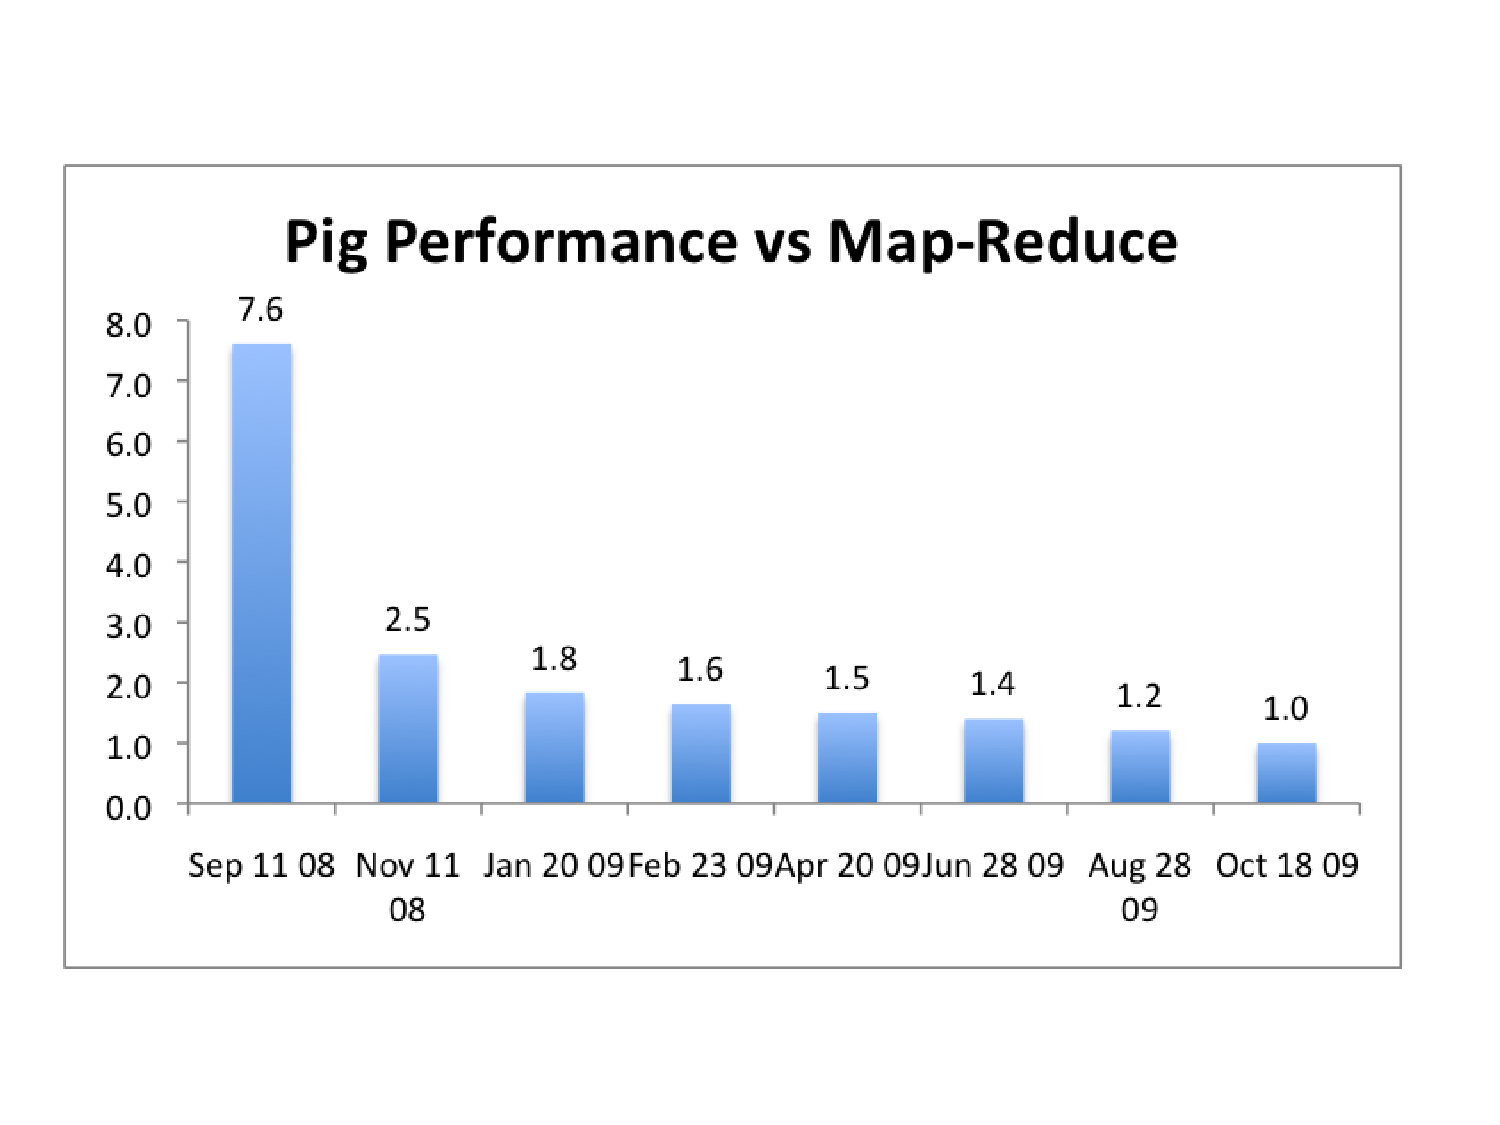
\includegraphics[scale=0.5]{./Figures/pig_perf}
  \end{figure}
}


%%%%%%%%%%%%%%%%%%%%%%%%%%%%%%%%%%%%%%%%%%%%%%%%%%%%%%%%%%
%%%%%%%%%%%%%%%%%%%%%%%%%%%%%%%%%%%%%%%%%%%%%%%%%%%%%%%%%%
\subsection{Pig Latin}
%%%%%%%%%%%%%%%%%%%%%%%%%%%%%%%%%%%%%%%%%%%%%%%%%%%%%%%%%%
%%%%%%%%%%%%%%%%%%%%%%%%%%%%%%%%%%%%%%%%%%%%%%%%%%%%%%%%%%

\begin{frame}
 \begin{colorblock}{blue}{lightblue}{ }
  \begin{center}
    \Huge \textbf{\texttt{Pig Latin}}
  \end{center}
  \end{colorblock}
\end{frame}


%%%%%%%%%%%%%%%%%%%%%%%%%%%%%%%%%%%%%%%%%%%%%%%%%%%%%%%%%%
\frame {\frametitle{Introduction}
%%%%%%%%%%%%%%%%%%%%%%%%%%%%%%%%%%%%%%%%%%%%%%%%%%%%%%%%%%
  \begin{itemize}
  \item \textbf{Not a complete reference to the Pig Latin language}:
    refer to \cite{pig}
    \begin{itemize}
    \item Here we cover some interesting/useful aspects
    \end{itemize}

    \vspace{20pt}

  \item \textbf{The focus here is on some language primitives}
    \begin{itemize}
    \item Optimizations are treated separately
    \item How they can be implemented (in the underlying engine) is not covered
    \end{itemize}

    \vspace{20pt}

  \item \textbf{Examples are taken from \cite{Olston2008, White2010}}
  \end{itemize}
}

%%%%%%%%%%%%%%%%%%%%%%%%%%%%%%%%%%%%%%%%%%%%%%%%%%%%%%%%%%
\frame {\frametitle{Data Model}
%%%%%%%%%%%%%%%%%%%%%%%%%%%%%%%%%%%%%%%%%%%%%%%%%%%%%%%%%%
  \begin{itemize}
  \item \textbf{Supports four types}
    \begin{itemize}
    \item \textit{Atom:} contains a simple atomic value as a string or
      a number, e.g. \texttt{`alice'}

      \vspace{20pt}

    \item \textit{Tuple:} sequence of \textit{fields}, each can be  of
      any data type, e.g., \texttt{(`alice', `lakers')}

      \vspace{20pt}

    \item \textit{Bag:} collection of tuples with possible
      duplicates. Flexible schema, no need to have the same number and
      type of fields


      \begin{tabular}{@{}l}
        $\left\{
          \begin{tabular}{@{}*1{c}}
            \texttt{(`alice',`lakers')} \\
            \texttt{(`alice',(`iPod',`apple'))}
          \end{tabular}
        \right\}$
      \end{tabular}

      \vspace{10pt}

      The example shows that tuples can be nested
    \end{itemize}
  \end{itemize}
}

%%%%%%%%%%%%%%%%%%%%%%%%%%%%%%%%%%%%%%%%%%%%%%%%%%%%%%%%%%
\frame {\frametitle{Data Model}
%%%%%%%%%%%%%%%%%%%%%%%%%%%%%%%%%%%%%%%%%%%%%%%%%%%%%%%%%%
  \begin{itemize}
  \item \textbf{Supports four types}
    \begin{itemize}

    \item \textit{Map:} collection of data items, where each item has
      an associated key for lookup. The schema, as with bags, is
      flexible.
      \begin{itemize}
      \item {\color{red}NOTE:} keys are required to be data atoms, for
        efficient lookup.
      \end{itemize}

      \vspace{10pt}

      \begin{tabular}{@{}l}
        $\left [
          \begin{tabular}{@{}*1{c}}
            \texttt{`fan of' $\to$  $\left\{
              \begin{tabular}{@{}*1{c}}
                (`lakers')\\
                (`iPod')
              \end{tabular} \right\}$
            } \\
            \texttt{`age' $\to$ 20}
          \end{tabular}
        \right ]$
      \end{tabular}

      \vspace{10pt}

      \begin{itemize}
      \item The key \texttt{`fan of'} is mapped to a bag containing two
        tuples
      \item The key \texttt{`age'} is mapped to an atom
      \end{itemize}

    \item Maps are useful to model datasets in which schema may be
      dynamic (over time)
    \end{itemize}
  \end{itemize}
}

%%%%%%%%%%%%%%%%%%%%%%%%%%%%%%%%%%%%%%%%%%%%%%%%%%%%%%%%%%
\frame {\frametitle{Structure}
%%%%%%%%%%%%%%%%%%%%%%%%%%%%%%%%%%%%%%%%%%%%%%%%%%%%%%%%%%
  \begin{itemize}
  \item \textbf{Pig Latin programs are a sequence of steps}
    \begin{itemize}
    \item Can use an interactive shell (called \texttt{grunt})
    \item Can feed them as a ``script''
    \end{itemize}

    \vspace{20pt}

  \item \textbf{Comments}
    \begin{itemize}
    \item In line: with double hyphens (\texttt{- -})
    \item C-style for longer comments (\texttt{/* ... */})
    \end{itemize}

    \vspace{20pt}

  \item \textbf{Reserved keywords}
    \begin{itemize}
    \item List of keywords that can't be used as identifiers
    \item Same old story as for any language
    \end{itemize}

  \end{itemize}
}

%%%%%%%%%%%%%%%%%%%%%%%%%%%%%%%%%%%%%%%%%%%%%%%%%%%%%%%%%%
\frame {\frametitle{Statements}
  \begin{itemize}
  \item \textbf{As a Pig Latin program is executed, each statement is
      \textit{parsed}} 
    \begin{itemize}
    \item The interpreter builds a \textbf{{\color{red}logical plan}} for every
      relational operation
    \item The logical plan of each statement is added to that of the
      program so far
    \item Then the interpreter moves on to the next statement
    \end{itemize}

    \vspace{20pt}

  \item \textbf{{\color{red}IMPORTANT:} No data processing takes place during
      construction of logical plan} $\to$ \textbf{{\color{red}Lazy Evaluation}}
    \begin{itemize}
    \item When the interpreter sees the first line of a program, it
      confirms that it is syntactically and semantically correct
    \item Then it adds it to the logical plan
    \item It does not even check the existence of files, for data load operations
    \end{itemize}
  \end{itemize}
}

%%%%%%%%%%%%%%%%%%%%%%%%%%%%%%%%%%%%%%%%%%%%%%%%%%%%%%%%%%
\frame {\frametitle{Statements}
%%%%%%%%%%%%%%%%%%%%%%%%%%%%%%%%%%%%%%%%%%%%%%%%%%%%%%%%%%
  \begin{itemize}
  \item[$\to$] \textbf{It makes no sense to start any processing until the
      whole flow is defined}
    \begin{itemize}
    \item Indeed, there are several optimizations that could make a
      program more efficient (e.g., by avoiding to operate on some
      data that later on is going to be filtered)
    \end{itemize}

    \vspace{20pt}

  \item \textbf{The trigger for Pig to start execution are the
      \texttt{DUMP} and \texttt{STORE} statements} 
    \begin{itemize}
    \item It is only at this point that the logical plan is
      {\color{red}compiled} into a {\color{red}physical plan}
    \end{itemize}

    \vspace{20pt}

  \item \textbf{How the physical plan is built}
    \begin{itemize}
    \item Pig prepares a series of MapReduce jobs
      \begin{itemize}
      \item In \textit{Local mode}, these are run locally on the JVM
      \item In \textit{MapReduce mode}, the jobs are sent to the
        Hadoop Cluster
      \end{itemize}
    \item {\color{red}IMPORTANT:} The command \texttt{EXPLAIN} can be used to show the MapReduce plan
    \end{itemize}
  \end{itemize}
}

%%%%%%%%%%%%%%%%%%%%%%%%%%%%%%%%%%%%%%%%%%%%%%%%%%%%%%%%%%
\frame {\frametitle{Statements}
%%%%%%%%%%%%%%%%%%%%%%%%%%%%%%%%%%%%%%%%%%%%%%%%%%%%%%%%%%
  \begin{beamerboxesrounded}{}
	\begin{center}
          Multi-query execution
	\end{center}    
  \end{beamerboxesrounded}

  \begin{itemize}
  \item \textbf{There is a difference between \texttt{DUMP} and \texttt{STORE}}
    \begin{itemize}
    \item Apart from diagnosis, and interactive mode, in batch mode
      \texttt{STORE} allows for program/job optimizations
    \end{itemize}

    \vspace{20pt}

  \item \textbf{Main optimization objective: minimize I/O}
    \begin{itemize}
    \item Consider the following example:
    \item[] \texttt{A = LOAD 'input/pig/multiquery/A';}
    \item[] \texttt{B = FILTER A BY \$1 == 'banana';}
    \item[] \texttt{C = FILTER A BY \$1 != 'banana';}
    \item[] \texttt{STORE B INTO 'output/b';}
    \item[] \texttt{STORE C INTO 'output/c';}
    \end{itemize}

  \end{itemize}
}

%%%%%%%%%%%%%%%%%%%%%%%%%%%%%%%%%%%%%%%%%%%%%%%%%%%%%%%%%%
\frame {\frametitle{Statements}
%%%%%%%%%%%%%%%%%%%%%%%%%%%%%%%%%%%%%%%%%%%%%%%%%%%%%%%%%%
  \begin{beamerboxesrounded}{}
	\begin{center}
          Multi-query execution
	\end{center}    
  \end{beamerboxesrounded}

  \begin{itemize}
  \item \textbf{In the example, relations \texttt{B} and \texttt{C} are both
      derived from \texttt{A}}
    \begin{itemize}
    \item Naively, this means that at the first \texttt{STORE}
      operator the input should be read
    \item Then, at the second \texttt{STORE} operator, the input
      should be read again 
    \end{itemize}

    \vspace{20pt}

  \item \textbf{Pig will run this as a single MapReduce job}
    \begin{itemize}
    \item Relation \texttt{A} is going to be read only once
    \item Then, each relation \texttt{B} and \texttt{C} will be
      written to the output 
    \end{itemize}

  \end{itemize}

}

%%%%%%%%%%%%%%%%%%%%%%%%%%%%%%%%%%%%%%%%%%%%%%%%%%%%%%%%%%
\frame {\frametitle{Expressions}
%%%%%%%%%%%%%%%%%%%%%%%%%%%%%%%%%%%%%%%%%%%%%%%%%%%%%%%%%%
  \begin{itemize}
  \item \textbf{An expression is something that is evaluated to yield
      a value}
    \begin{itemize}
    \item Lookup on \cite{White2010} for documentation
    \end{itemize}
  \end{itemize}
  \begin{figure}[h]
    \centering
    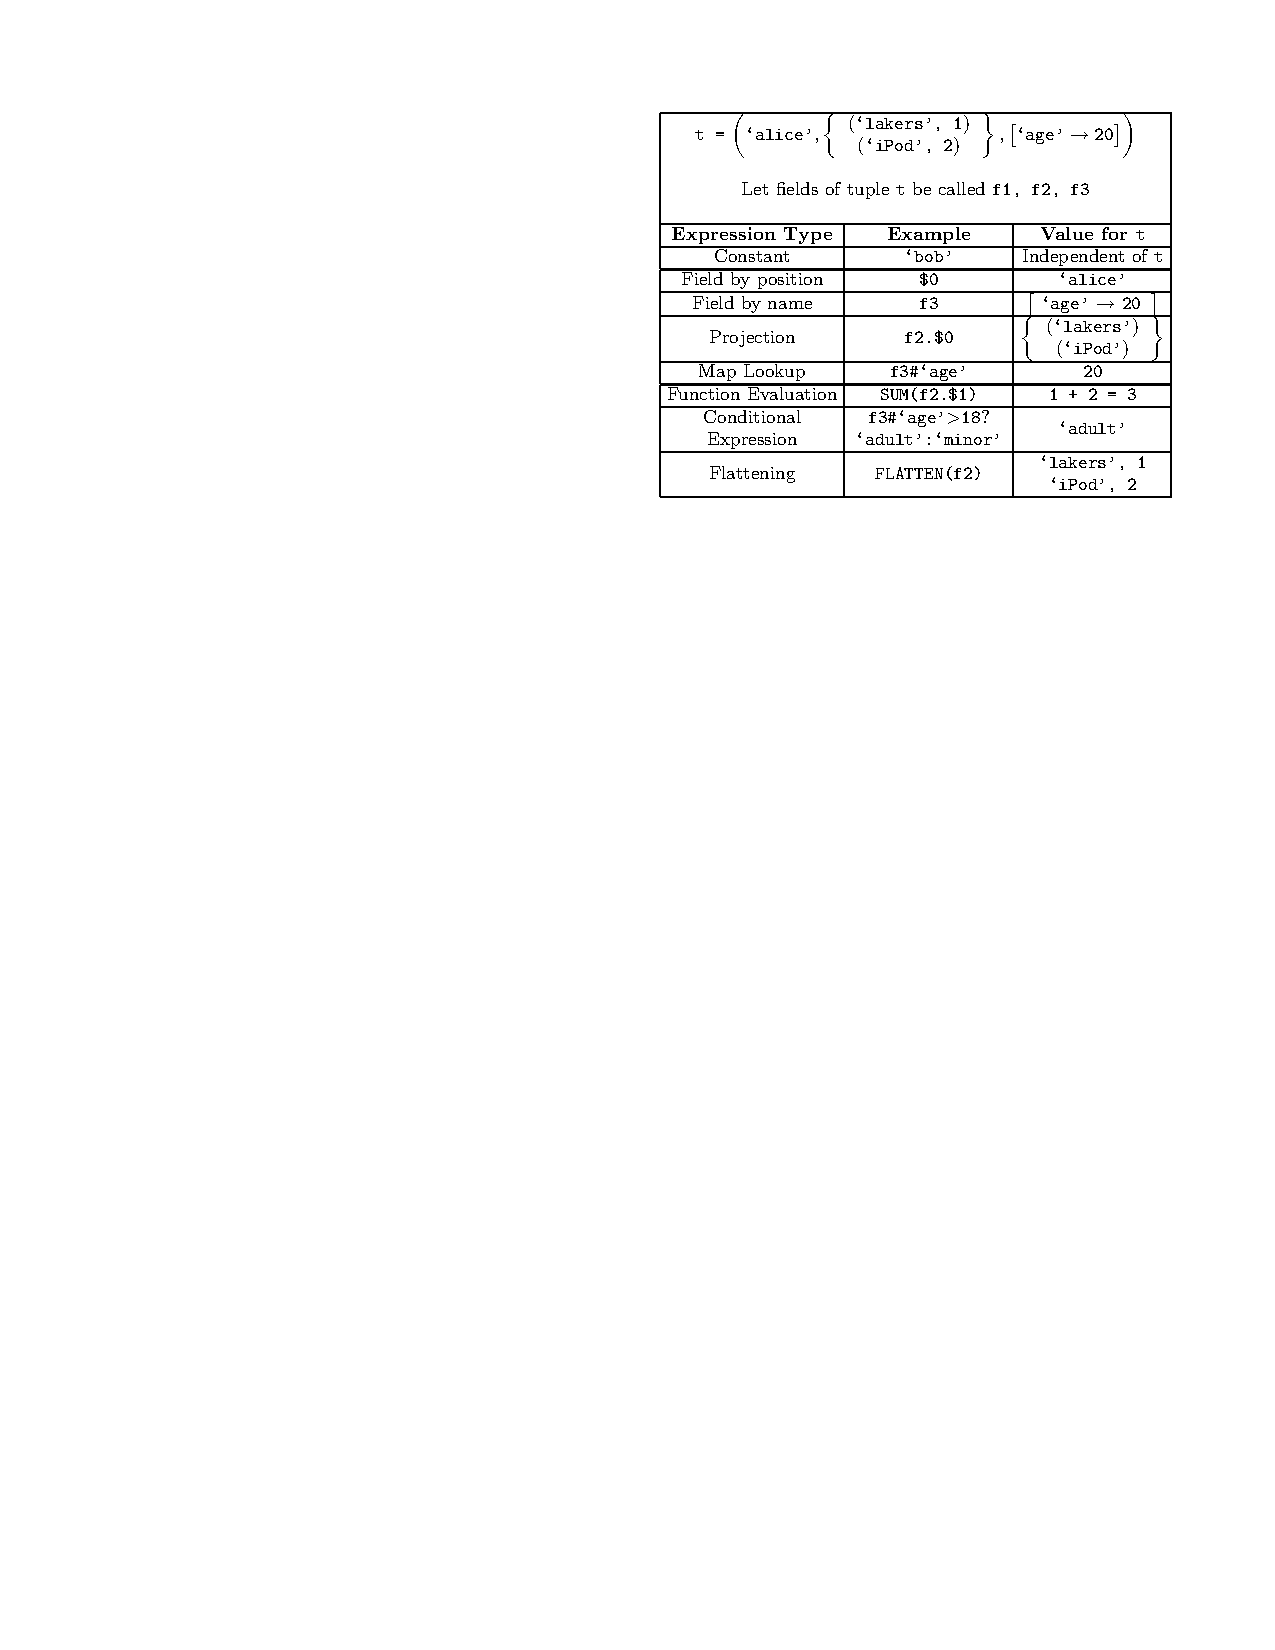
\includegraphics[scale=0.9]{./Figures/expressions}
  \end{figure}
}

%%%%%%%%%%%%%%%%%%%%%%%%%%%%%%%%%%%%%%%%%%%%%%%%%%%%%%%%%%
\frame {\frametitle{Schemas}
  \begin{itemize}
  \item \textbf{A relation in Pig may have an associated schema}
    \begin{itemize}
    \item This is optional
    \item A schema gives the fields in the relations names and types
    \item Use the command \texttt{DESCRIBE} to reveal the schema in
      use for a relation
    \end{itemize}
    
    \vspace{20pt}
    
  \item \textbf{Schema declaration is flexible but reuse is awkward}\footnote{Current developments solve this problem: HCatalogs. We will not cover this in this course.}
    \begin{itemize}
    \item A set of queries over the same input data will often have
      the same schema
    \item This is sometimes hard to maintain (unlike HIVE) as there is no
      external components to maintain this association
    \item[HINT::] You can write a UDF to perform a
      personalized load operation which encapsulates the schema
    \end{itemize}

  \end{itemize}
}

%%%%%%%%%%%%%%%%%%%%%%%%%%%%%%%%%%%%%%%%%%%%%%%%%%%%%%%%%%
\frame {\frametitle{Validation and nulls}
%%%%%%%%%%%%%%%%%%%%%%%%%%%%%%%%%%%%%%%%%%%%%%%%%%%%%%%%%%
  \begin{itemize}
  \item \textbf{Pig does not have the same power to enforce constraints on
      schema at load time as a RDBMS}
    \begin{itemize}
    \item If a value cannot be cast to a type declared in the schema,
      then it will be set to a \texttt{null} value
    \item This also happens for corrupt files
    \end{itemize}

    \vspace{10pt}
    
  \item \textbf{A useful technique to partition input data to discern
      good and bad records}
    \begin{itemize}
    \item Use the \texttt{SPLIT} operator
    \item[] \texttt{SPLIT records INTO good\_records IF temperature is not
      null, bad \_records IF temperature is NULL;}
    \end{itemize}
  \end{itemize}

}

%%%%%%%%%%%%%%%%%%%%%%%%%%%%%%%%%%%%%%%%%%%%%%%%%%%%%%%%%%
\frame {\frametitle{Other relevant information}
%%%%%%%%%%%%%%%%%%%%%%%%%%%%%%%%%%%%%%%%%%%%%%%%%%%%%%%%%%
  \begin{itemize}
  \item \textbf{Schema propagation and merging}
    \begin{itemize}
    \item How schema are propagated to new relations?
    \item Advanced, but important topic
    \end{itemize}

    \vspace{20pt}
        
  \item \textbf{User-Defined Functions}
    \begin{itemize}
    \item Use \cite{White2010} for an introduction to designing UDFs
    \end{itemize}
  \end{itemize}
}

%%%%%%%%%%%%%%%%%%%%%%%%%%%%%%%%%%%%%%%%%%%%%%%%%%%%%%%%%%
\frame {\frametitle{Data Processing Operators}
%%%%%%%%%%%%%%%%%%%%%%%%%%%%%%%%%%%%%%%%%%%%%%%%%%%%%%%%%%
  \begin{beamerboxesrounded}{}
	\begin{center}
          Loading and storing data
	\end{center}    
  \end{beamerboxesrounded}

  \begin{itemize}
  \item \textbf{The first step in a Pig Latin program is to load data}
    \begin{itemize}
    \item Accounts for what input files are (e.g. csv files)
    \item How the file contents are to be deserialized
    \item An input file is assumed to contain a sequence of tuples
    \end{itemize}

    \vspace{20pt}

  \item Data loading is done with the \texttt{LOAD} command
    \begin{itemize}
    \item[] \texttt{queries = LOAD `query\_log.txt'}
    \item[] \texttt{USING myLoad()}
    \item[] \texttt{AS (userId, queryString, timestamp);}
    \end{itemize}
  \end{itemize}
}

%%%%%%%%%%%%%%%%%%%%%%%%%%%%%%%%%%%%%%%%%%%%%%%%%%%%%%%%%%
\frame {\frametitle{Data Processing Operators}
%%%%%%%%%%%%%%%%%%%%%%%%%%%%%%%%%%%%%%%%%%%%%%%%%%%%%%%%%%
  \begin{beamerboxesrounded}{}
	\begin{center}
          Loading and storing data
	\end{center}    
  \end{beamerboxesrounded}

  \begin{itemize}
  \item \textbf{The example above specifies the following:}
    \begin{itemize}
    \item The input file is \texttt{query\_log.txt}
    \item The input file should be converted into tuples using the
      custom \texttt{myLoad} deserializer
    \item The loaded tuples have three fields, specified by the schema
    \end{itemize}

    \vspace{20pt}

  \item \textbf{Optional parts}
    \begin{itemize}
    \item \texttt{USING} clause is optional: if not specified, the
      input file is assumed to be plain text, tab-delimited
    \item \texttt{AS} clause is optional: if not specified, must refer
      to fileds by position instead of by name
    \end{itemize}

  \end{itemize}
}

%%%%%%%%%%%%%%%%%%%%%%%%%%%%%%%%%%%%%%%%%%%%%%%%%%%%%%%%%%
\frame {\frametitle{Data Processing Operators}
%%%%%%%%%%%%%%%%%%%%%%%%%%%%%%%%%%%%%%%%%%%%%%%%%%%%%%%%%%
  \begin{beamerboxesrounded}{}
	\begin{center}
          Loading and storing data
	\end{center}    
  \end{beamerboxesrounded}

  \begin{itemize}
  \item Return value of the \texttt{LOAD} command
    \begin{itemize}
    \item Handle to a bag
    \item This can be used by subsequent commands
    \item[$\to$] bag handles are only logical
    \item[$\to$] no file is actually read!
    \end{itemize}  

    \vspace{20pt}
    
  \item The command to write output to disk is \texttt{STORE}
    \begin{itemize}
    \item It has similar semantics to the \texttt{LOAD} command
    \end{itemize}
  \end{itemize}
}

%%%%%%%%%%%%%%%%%%%%%%%%%%%%%%%%%%%%%%%%%%%%%%%%%%%%%%%%%%
\frame {\frametitle{Data Processing Operators}
%%%%%%%%%%%%%%%%%%%%%%%%%%%%%%%%%%%%%%%%%%%%%%%%%%%%%%%%%%
  \begin{beamerboxesrounded}{}
  \begin{center}
          Loading and storing data: Example
  \end{center}    
  \end{beamerboxesrounded}

\begin{itemize}
  \item[] \texttt{A = LOAD 'myfile.txt' USING PigStorage(',') AS (f1,f2,f3);}
  \item[] 
  \item[] \texttt{<1, 2, 3>}
  \item[] \texttt{<4, 2, 1>}
  \item[] \texttt{<8, 3, 4>}
  \item[] \texttt{<4, 3, 3>}
  \item[] \texttt{<7, 2, 5>}
  \item[] \texttt{<8, 4, 3>}
\end{itemize}
}


%%%%%%%%%%%%%%%%%%%%%%%%%%%%%%%%%%%%%%%%%%%%%%%%%%%%%%%%%%
\frame {\frametitle{Data Processing Operators}
%%%%%%%%%%%%%%%%%%%%%%%%%%%%%%%%%%%%%%%%%%%%%%%%%%%%%%%%%%
  \begin{beamerboxesrounded}{}
	\begin{center}
          Per-tuple processing
	\end{center}    
  \end{beamerboxesrounded}

  \begin{itemize}
  \item \textbf{Once you have some data loaded into a relation, a possible next step is, e.g.,  to filter it}
    \begin{itemize}
    \item This is done, e.g., to remove unwanted data
    \item {\color{red}HINT:} By filtering early in the processing
      pipeline, you minimize the amount of data flowing trough the system
    \end{itemize}

    \vspace{20pt}

  \item \textbf{A basic operation is to apply some processing over every tuple
      of a data set}
    \begin{itemize}
    \item This is achieved with the \texttt{FOREACH} command
    \item[] \texttt{expanded\_queries = FOREACH queries GENERATE}
    \item[] \texttt{userId, expandQuery(queryString);}
    \end{itemize}
  \end{itemize}
  
}

%%%%%%%%%%%%%%%%%%%%%%%%%%%%%%%%%%%%%%%%%%%%%%%%%%%%%%%%%%
\frame {\frametitle{Data Processing Operators}
%%%%%%%%%%%%%%%%%%%%%%%%%%%%%%%%%%%%%%%%%%%%%%%%%%%%%%%%%%
  \begin{beamerboxesrounded}{}
	\begin{center}
          Per-tuple processing
	\end{center}    
  \end{beamerboxesrounded}

  \begin{itemize}
  \item \textbf{Comments on the example above:}
    \begin{itemize}
    \item Each tuple of the bag \texttt{queries} should be processed
      {\color{red}independently}
    \item The second field of the output is the result of a UDF
    \end{itemize}

    \vspace{20pt}

  \item \textbf{Semantics of the \texttt{FOREACH} command}
    \begin{itemize}
    \item There can be no dependence between the processing of
      different input tuples
    \item[$\to$] This allows for an efficient parallel implementation
    \end{itemize}

    \vspace{20pt}

    \item \textbf{Semantics of the \texttt{GENERATE} clause}
      \begin{itemize}
      \item Followed by a list of expressions
      \item Also \textit{flattening} is allowed
        \begin{itemize}
        \item This is done to eliminate nesting in data
        \item[$\to$] Allows to make output data independent for
          further parallel processing
        \item[$\to$] Useful to store data on disk
        \end{itemize}
      \end{itemize}

  \end{itemize}
}

%%%%%%%%%%%%%%%%%%%%%%%%%%%%%%%%%%%%%%%%%%%%%%%%%%%%%%%%%%
\frame {\frametitle{Data Processing Operators}
%%%%%%%%%%%%%%%%%%%%%%%%%%%%%%%%%%%%%%%%%%%%%%%%%%%%%%%%%%
  \begin{beamerboxesrounded}{}
  \begin{center}
          Per-tuple processing: example
  \end{center}    
  \end{beamerboxesrounded}

\begin{itemize}
  \item[] \texttt{X = FOREACH A GENERATE f0, f1+f2;}
  \item[] \texttt{Y = GROUP A BY f0;}
  \item[] \texttt{Z = FOREACH Y GENERATE group, Y.(\$1, \$2);} 
\end{itemize}

  \begin{columns}
    \begin{column}{.3\linewidth}
    \begin{itemize}
      \item[] \texttt{A=}
      \item[] \texttt{<1, 2, 3>}
      \item[] \texttt{<4, 2, 1>}
      \item[] \texttt{<8, 3, 4>}
      \item[] \texttt{<4, 3, 3>}
      \item[] \texttt{<7, 2, 5>}
      \item[] \texttt{<8, 4, 3>}
    \end{itemize}
    \end{column}

    \begin{column}{.2\linewidth}
    \begin{itemize}
      \item[] \texttt{X=}
      \item[] \texttt{<1, 5>}
      \item[] \texttt{<4, 3>}
      \item[] \texttt{<8, 7>}
      \item[] \texttt{<4, 6>}
      \item[] \texttt{<7, 7>}
      \item[] \texttt{<8, 7>}
    \end{itemize}
    \end{column}

    \begin{column}{.5\linewidth}
    \begin{footnotesize}
    \begin{itemize}
      \item[] \texttt{Z=}
      \item[] \texttt{<1, \{<2, 3>\}>}
      \item[] \texttt{<4, \{<2, 1>, <3, 3>\}>}
      \item[] \texttt{<7, \{<2, 5>\}>}
      \item[] \texttt{<8, \{<3, 4>, <4, 3>\}>}
    \end{itemize}
    \end{footnotesize}
    \end{column}
  \end{columns}
}

%%%%%%%%%%%%%%%%%%%%%%%%%%%%%%%%%%%%%%%%%%%%%%%%%%%%%%%%%%
\frame {\frametitle{Data Processing Operators}
%%%%%%%%%%%%%%%%%%%%%%%%%%%%%%%%%%%%%%%%%%%%%%%%%%%%%%%%%%
  \begin{beamerboxesrounded}{}
	\begin{center}
          Per-tuple processing: Discarding unwanted data
	\end{center}    
  \end{beamerboxesrounded}

  \begin{itemize}
  \item \textbf{A common operation is to retain a portion of the input
      data}
    \begin{itemize}
    \item This is done with the \texttt{FILTER} command
    \item[] \texttt{real\_queries = FILTER queries BY userId neq `bot';}
    \end{itemize}

    \vspace{20pt}

  \item \textbf{Filtering conditions involve a combination of
      expressions}
    \begin{itemize}
    \item Comparison operators
    \item Logical connectors
    \item UDF 
    \end{itemize}
  \end{itemize}
}

%%%%%%%%%%%%%%%%%%%%%%%%%%%%%%%%%%%%%%%%%%%%%%%%%%%%%%%%%%
\frame {\frametitle{Data Processing Operators}
%%%%%%%%%%%%%%%%%%%%%%%%%%%%%%%%%%%%%%%%%%%%%%%%%%%%%%%%%%
  \begin{beamerboxesrounded}{}
  \begin{center}
          Filtering: example
  \end{center}    
  \end{beamerboxesrounded}

\begin{itemize}
  \item[] \texttt{Y = FILTER A BY f1 == '8';} 
\end{itemize}

  \begin{columns}
    \begin{column}{.5\linewidth}
    \begin{itemize}
      \item[] \texttt{A=}
      \item[] \texttt{<1, 2, 3>}
      \item[] \texttt{<4, 2, 1>}
      \item[] \texttt{<8, 3, 4>}
      \item[] \texttt{<4, 3, 3>}
      \item[] \texttt{<7, 2, 5>}
      \item[] \texttt{<8, 4, 3>}
    \end{itemize}
    \end{column}

    \begin{column}{.5\linewidth}
    \begin{itemize}
      \item[] \texttt{Y=}
      \item[] \texttt{<8, 3, 4>}
      \item[] \texttt{<8, 4, 3>}
    \end{itemize}

    \end{column}
  \end{columns}
}

%%%%%%%%%%%%%%%%%%%%%%%%%%%%%%%%%%%%%%%%%%%%%%%%%%%%%%%%%%
\frame {\frametitle{Data Processing Operators}
%%%%%%%%%%%%%%%%%%%%%%%%%%%%%%%%%%%%%%%%%%%%%%%%%%%%%%%%%%
  \begin{beamerboxesrounded}{}
	\begin{center}
          Per-tuple processing: Streaming data
	\end{center}    
  \end{beamerboxesrounded}

  \begin{itemize}
  \item \textbf{The \texttt{STREAM} operator allows transforming data in a
      relation using an external program or script}
    \begin{itemize}
    \item This is possible because Hadoop MapReduce supports
      ``streaming''
    \item Example:
    \item[] \texttt{C = STREAM A THROUGH `cut -f 2';}
    \item[] which use the Unix \texttt{cut} command to extract the
      second filed of each tuple in \texttt{A}
    \end{itemize}

    \vspace{20pt}

  \item \textbf{The \texttt{STREAM} operator uses \texttt{PigStorage} to
    serialize and deserialize relations to and from \texttt{stdin/stdout}}
    \begin{itemize}
    \item Can also provide a custom serializer/deserializer
    \item Works well with python
    \end{itemize}
  \end{itemize}


}

%%%%%%%%%%%%%%%%%%%%%%%%%%%%%%%%%%%%%%%%%%%%%%%%%%%%%%%%%%
\frame {\frametitle{Data Processing Operators}
%%%%%%%%%%%%%%%%%%%%%%%%%%%%%%%%%%%%%%%%%%%%%%%%%%%%%%%%%%
  \begin{beamerboxesrounded}{}
	\begin{center}
          Getting related data together
	\end{center}    
  \end{beamerboxesrounded}

  \begin{itemize}
  \item \textbf{It is often necessary to \textit{group} together tuples from one or more data sets}
    \begin{itemize}
    \item We will explore several nuances of ``grouping''
    \end{itemize}

    % \vspace{20pt}

  % \item \textbf{A grouping operation we study in details is the COGROUP command}
  % \item[] Example: Assume we have loaded two relations from a Search Engine log file
  % \item[] \texttt{results: (queryString, url, position)}
  % \item[] \texttt{revenue: (queryString, adSlot, amount)}
  %   \begin{itemize}
  %   \item \texttt{results} contains, for different query strings, the
  %     urls shown as search results, and the positions at which they
  %     where shown
  %   \item \texttt{revenue} contains, for different query strings, and
  %     different advertisement slots, the average amount of revenue
  %   \end{itemize}

  \end{itemize}
}

%%%%%%%%%%%%%%%%%%%%%%%%%%%%%%%%%%%%%%%%%%%%%%%%%%%%%%%%%%
\frame {\frametitle{Data Processing Operators}
%%%%%%%%%%%%%%%%%%%%%%%%%%%%%%%%%%%%%%%%%%%%%%%%%%%%%%%%%%
  \begin{beamerboxesrounded}{}
  \begin{center}
          The \texttt{GROUP} operator
  \end{center}    
  \end{beamerboxesrounded}

  \begin{itemize}
  \item \textbf{Sometimes, we want to operate on a single dataset}
    \begin{itemize}
    \item This is when you use the \texttt{GROUP} operator
    \end{itemize}

    \vspace{20pt}

  \item \textbf{Let's continue from Example 3:}
    \begin{itemize}
    \item Assume we want to find the total revenue for each query
      string. This writes as:
    \item[] \texttt{grouped\_revenue = GROUP revenue BY queryString;}
    \item[] \texttt{query\_revenue = FOREACH grouped\_revenue GENERATE}
    \item[] \texttt{queryString, SUM(revenue.amount) AS totalRevenue;}

      \vspace{10pt}

  \item Note that \texttt{revenue.amount} refers to a projection of
    the nested bag in the tuples of \texttt{grouped\_revenue}

    \end{itemize}
  \end{itemize}
}

%%%%%%%%%%%%%%%%%%%%%%%%%%%%%%%%%%%%%%%%%%%%%%%%%%%%%%%%%%
\frame {\frametitle{Data Processing Operators}
%%%%%%%%%%%%%%%%%%%%%%%%%%%%%%%%%%%%%%%%%%%%%%%%%%%%%%%%%%
  \begin{beamerboxesrounded}{}
  \begin{center}
          \texttt{GROUP ... BY ...}: Example
  \end{center}    
  \end{beamerboxesrounded}

\begin{itemize}
  \item[] \texttt{X = GROUP A BY f1;} 
\end{itemize}

  \begin{columns}
    \begin{column}{.3\linewidth}
    \begin{itemize}
      \item[] \texttt{A=}
      \item[] \texttt{<1, 2, 3>}
      \item[] \texttt{<4, 2, 1>}
      \item[] \texttt{<8, 3, 4>}
      \item[] \texttt{<4, 3, 3>}
      \item[] \texttt{<7, 2, 5>}
      \item[] \texttt{<8, 4, 3>}
    \end{itemize}
    \end{column}

    \begin{column}{.7\linewidth}
    \begin{footnotesize}
    \begin{itemize}
      \item[] \texttt{X=}
      \item[] \texttt{<1, {<1, 2, 3>}>}
      \item[] \texttt{<4, {<4, 2, 1>, <4, 3, 3>}>}
      \item[] \texttt{<7, {<7, 2, 5>}>}
      \item[] \texttt{<8, {<8, 3, 4>, <8, 4, 3>}>}
    \end{itemize}
    \end{footnotesize}
    \end{column}
  \end{columns}
}

%%%%%%%%%%%%%%%%%%%%%%%%%%%%%%%%%%%%%%%%%%%%%%%%%%%%%%%%%%
\frame {\frametitle{Data Processing Operators}
%%%%%%%%%%%%%%%%%%%%%%%%%%%%%%%%%%%%%%%%%%%%%%%%%%%%%%%%%%
  \begin{beamerboxesrounded}{}
	\begin{center}
          Getting related data together
	\end{center}    
  \end{beamerboxesrounded}

  \begin{itemize}
  \item \textbf{Suppose we want to group together all search results data and
      revenue data for the same query string}
    \begin{itemize}
    \item[] \texttt{grouped\_data = COGROUP results BY queryString, revenue BY queryString;}
    \end{itemize}
  \end{itemize}

  \begin{figure}[h]
    \centering
    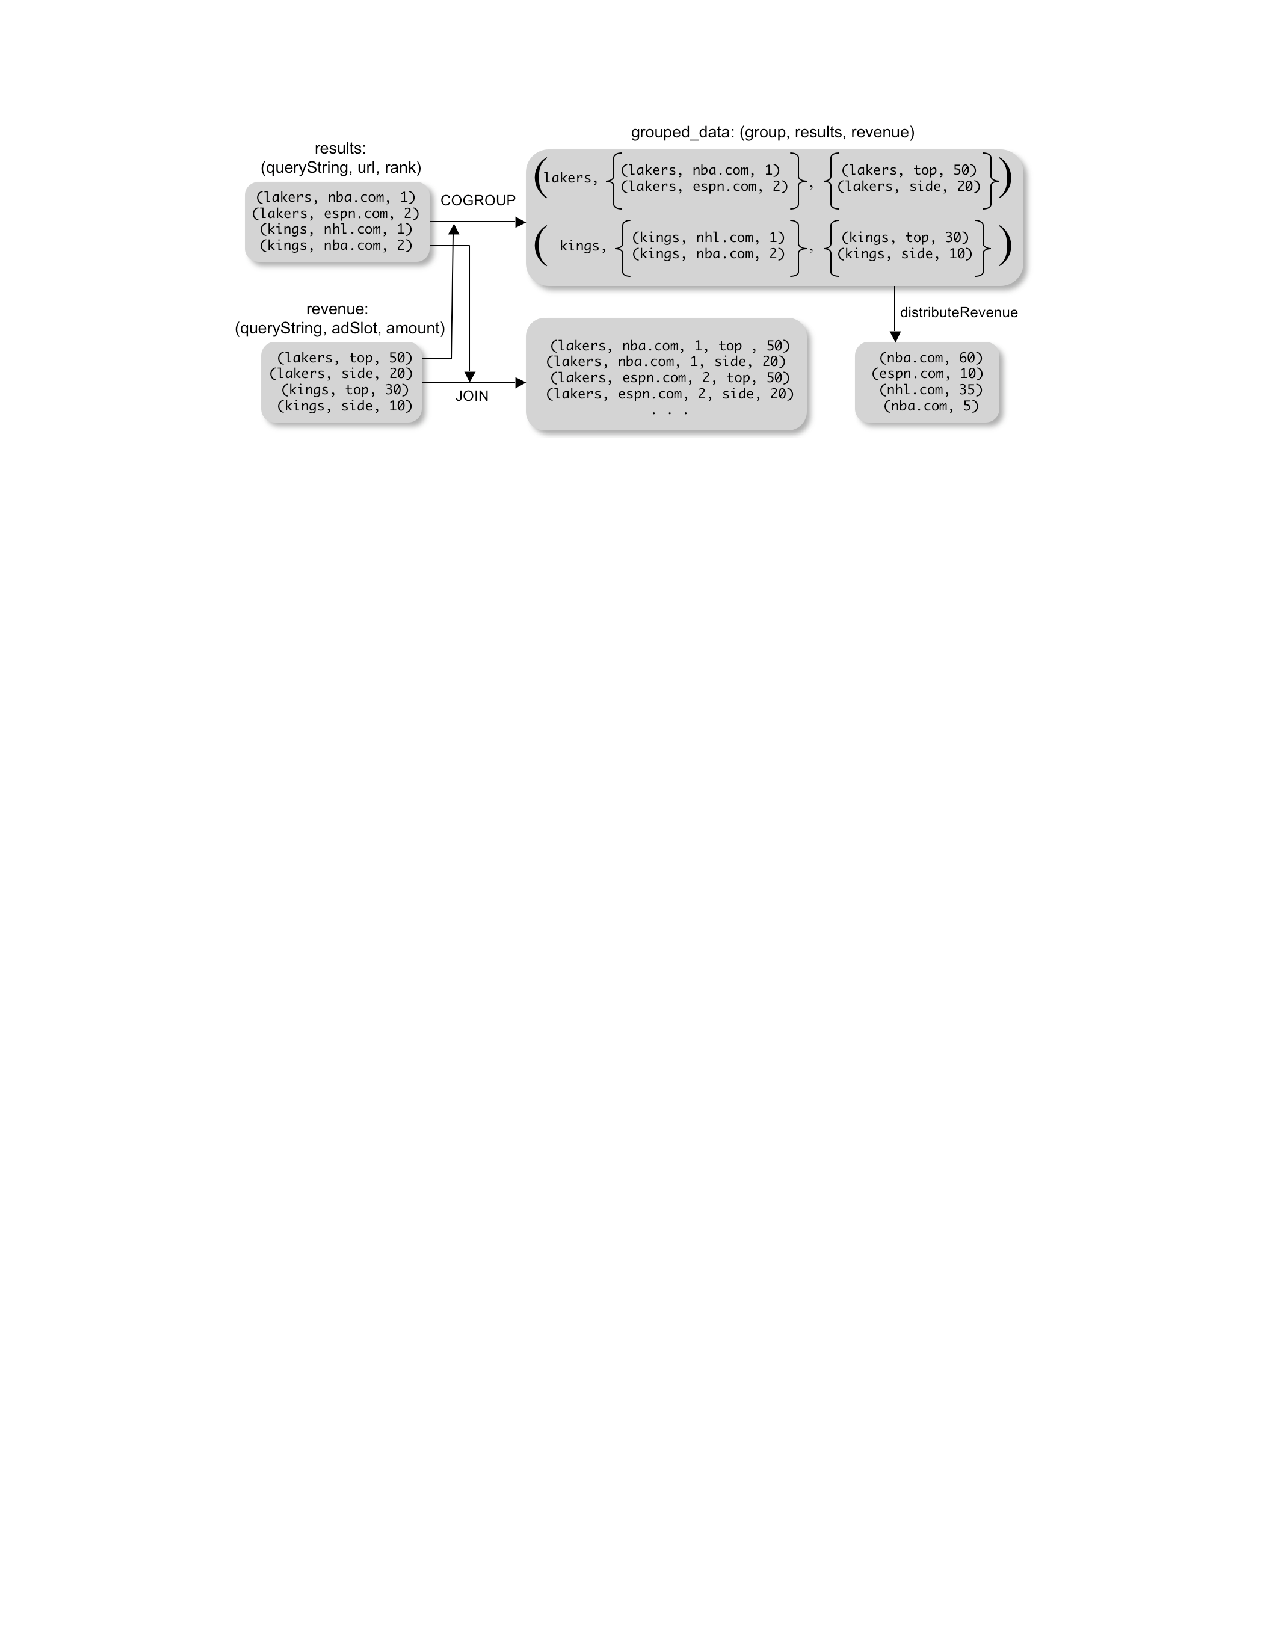
\includegraphics[scale=0.8]{./Figures/cogroup}
  \end{figure}
}

%%%%%%%%%%%%%%%%%%%%%%%%%%%%%%%%%%%%%%%%%%%%%%%%%%%%%%%%%%
\frame {\frametitle{Data Processing Operators}
%%%%%%%%%%%%%%%%%%%%%%%%%%%%%%%%%%%%%%%%%%%%%%%%%%%%%%%%%%
  \begin{beamerboxesrounded}{}
	\begin{center}
          The \texttt{COGROUP} command
	\end{center}    
  \end{beamerboxesrounded}

  \begin{itemize}
  \item \textbf{Output of a \texttt{COGROUP} contains one tuple for
      each group} 
    \begin{itemize}
    \item First field (\texttt{group}) is the group identifier (the
      value of the \texttt{queryString})
    \item Each of the next fields is a bag, one for each group being
      co-grouped
    \end{itemize}

    \vspace{20pt}

  \item \textbf{Grouping can be performed according to UDFs}

    \vspace{20pt}

  \item \textbf{Next: a clarifying example}
  \end{itemize}

}

%%%%%%%%%%%%%%%%%%%%%%%%%%%%%%%%%%%%%%%%%%%%%%%%%%%%%%%%%%
\frame {\frametitle{Data Processing Operators}
%%%%%%%%%%%%%%%%%%%%%%%%%%%%%%%%%%%%%%%%%%%%%%%%%%%%%%%%%%
  % \begin{beamerboxesrounded}{}
  % \begin{center}
  %         \texttt{COGROUP}: A Simple Example
  % \end{center}    
  % \end{beamerboxesrounded}

\begin{footnotesize}
\begin{itemize}
  \item[] \texttt{C = COGROUP A BY f1, B BY \$0;} 
\end{itemize}
\end{footnotesize}


  \begin{columns}
    \begin{column}{.5\linewidth}
    \begin{tiny}
    \begin{itemize}
      \item[] \texttt{A=}
      \item[] \texttt{<1, 2, 3>}
      \item[] \texttt{<4, 2, 1>}
      \item[] \texttt{<8, 3, 4>}
      \item[] \texttt{<4, 3, 3>}
      \item[] \texttt{<7, 2, 5>}
      \item[] \texttt{<8, 4, 3>}
    \end{itemize}
    \end{tiny}
    \end{column}

    \begin{column}{.5\linewidth}
    \begin{tiny}
    \begin{itemize}
      \item[] \texttt{B=}
      \item[] \texttt{<2, 4>}
      \item[] \texttt{<8, 9>}
      \item[] \texttt{<1, 3>}
      \item[] \texttt{<2, 7>}
      \item[] \texttt{<2, 9>}
      \item[] \texttt{<4, 6>}
      \item[] \texttt{<4, 9>}
    \end{itemize}
    \end{tiny}
    \end{column}
  \end{columns}

\begin{tiny}
\begin{itemize}
  \item[] \texttt{C=}
  \item[] \texttt{<1, \{<1, 2, 3>\}, \{<1, 3>\}>} 
  \item[] \texttt{<2, \{ \}, \{<2, 4>, <2, 7>, <2, 9>\}>} 
  \item[] \texttt{<4, \{<4, 2, 1>, <4, 3, 3>\}, \{<4, 6>,<4, 9>\}>}
  \item[] \texttt{<7, \{<7, 2, 5>\}, \{ \}>}
  \item[] \texttt{<8, \{<8, 3, 4>, <8, 4, 3>\}, \{<8, 9>\}>} 
\end{itemize}
\end{tiny}

}

%%%%%%%%%%%%%%%%%%%%%%%%%%%%%%%%%%%%%%%%%%%%%%%%%%%%%%%%%%
\frame {\frametitle{Data Processing Operators}
%%%%%%%%%%%%%%%%%%%%%%%%%%%%%%%%%%%%%%%%%%%%%%%%%%%%%%%%%%
  \begin{beamerboxesrounded}{}
	\begin{center}
          \texttt{COGROUP} vs \texttt{JOIN}
	\end{center}    
  \end{beamerboxesrounded}

  \begin{itemize}
  \item \texttt{JOIN} vs. \texttt{COGROUP}
    \begin{itemize}
    \item Their are equivalent: \texttt{JOIN} == \texttt{COGROUP}
      followed by a cross product of the tuples in the nested bags
    \end{itemize}

    \vspace{20pt}

  \item \textbf{Example 3: Suppose we try to attribute search revenue
      to search-results urls $\to$ compute monetary worth of each url}
    \begin{itemize}
    \item[] \texttt{grouped\_data = COGROUP results BY queryString,
        revenue BY queryString;}
      \item[] \texttt{url\_revenues = FOREACH grouped\_data GENERATE}
      \item[] \texttt{FLATTEN(distrubteRevenue(results, revenue));}

        \vspace{10pt}

      \item Where \texttt{distrubteRevenue} is a UDF that accepts
        search results and revenue information for each query string, and
        outputs a bag of urls and revenue attributed to them
    \end{itemize}

  \end{itemize}

}

%%%%%%%%%%%%%%%%%%%%%%%%%%%%%%%%%%%%%%%%%%%%%%%%%%%%%%%%%%
\frame {\frametitle{Data Processing Operators}
%%%%%%%%%%%%%%%%%%%%%%%%%%%%%%%%%%%%%%%%%%%%%%%%%%%%%%%%%%
  \begin{beamerboxesrounded}{}
	\begin{center}
          \texttt{COGROUP} vs \texttt{JOIN}
	\end{center}    
  \end{beamerboxesrounded}

  \begin{itemize}

  \item \textbf{More details on the UDF distribute Revenue}
    \begin{itemize}
    \item Attributes revenue from the top slot entirely to the first
      search result
    \item The revenue from the side slot may be equally split among
      all results
    \end{itemize}

    \vspace{20pt}

  \item \textbf{Let's see how to do the same with a \texttt{JOIN}}
    \begin{itemize}
    \item \texttt{JOIN} the tables \texttt{results} and
      \texttt{revenues} by \texttt{queryString}
    \item \texttt{GROUP BY} \texttt{queryString}
    \item Apply a custom aggregation function
    \end{itemize}

    \vspace{20pt}

  \item \textbf{What happens behind the scenes}
    \begin{itemize}
    \item During the \texttt{JOIN}, the system computes the cross product of
      the search and revenue information
    \item Then the custom aggregation needs to undo this cross
      product, because the UDF specifically requires so
    \end{itemize}
  \end{itemize}

}

%%%%%%%%%%%%%%%%%%%%%%%%%%%%%%%%%%%%%%%%%%%%%%%%%%%%%%%%%%
\frame {\frametitle{Data Processing Operators}
%%%%%%%%%%%%%%%%%%%%%%%%%%%%%%%%%%%%%%%%%%%%%%%%%%%%%%%%%%
  \begin{beamerboxesrounded}{}
	\begin{center}
          \texttt{COGROUP} in details
	\end{center}    
  \end{beamerboxesrounded}

  \begin{itemize}
  \item \textbf{The \texttt{COGROUP} statement conforms to an
      algebraic language}
    \begin{itemize}
    \item The operator carries out only the operation of grouping
      together tuples into nested bags
    \item The user can the decide whether to apply a (custom)
      aggregation on those tuples or to cross-product them and obtain
      a \texttt{JOIN}
    \end{itemize}

    \vspace{20pt}

  \item \textbf{It is thanks to the nested data model that \texttt{COGROUP} is
    an independent operation}
    \begin{itemize}
    \item Implementation details are tricky
    \item Groups can be very large (and are redundant)
    \end{itemize}
  \end{itemize}
}

%%%%%%%%%%%%%%%%%%%%%%%%%%%%%%%%%%%%%%%%%%%%%%%%%%%%%%%%%%
\frame {\frametitle{Data Processing Operators}
%%%%%%%%%%%%%%%%%%%%%%%%%%%%%%%%%%%%%%%%%%%%%%%%%%%%%%%%%%
  \begin{beamerboxesrounded}{}
	\begin{center}
          \texttt{JOIN} in Pig Latin
	\end{center}    
  \end{beamerboxesrounded}

  \begin{itemize}
  \item \textbf{In many cases, the typical operation on two or more datasets
      amounts to an equi-join}
    \begin{itemize}
    \item {\color{red}IMPORTANT NOTE:} large datasets that are
      suitable to be analyzed with Pig (and MapReduce) are generally
      \textbf{not normalized}
    \item[$\to$] \texttt{JOINs} are used more infrequently in Pig Latin than
      they are in SQL
    \end{itemize}

    \vspace{20pt}

  \item \textbf{The syntax of a \texttt{JOIN}}
    \begin{itemize}
    \item[] \texttt{join\_result = JOIN results BY queryString,
        revenue BY queryString;}

      \vspace{10pt}

    \item This is a classic inner join (actually an equi-join), where
      each match between the two relations corresponds to a row in the
      \texttt{join\_result} 
    \end{itemize}

  \end{itemize}
}

%%%%%%%%%%%%%%%%%%%%%%%%%%%%%%%%%%%%%%%%%%%%%%%%%%%%%%%%%%
\frame {\frametitle{Data Processing Operators}
%%%%%%%%%%%%%%%%%%%%%%%%%%%%%%%%%%%%%%%%%%%%%%%%%%%%%%%%%%
  \begin{beamerboxesrounded}{}
	\begin{center}
          \texttt{JOIN} in Pig Latin
	\end{center}    
  \end{beamerboxesrounded}

  \begin{itemize}
  \item \textbf{JOINs lend themselves to optimization opportunities}
    \begin{itemize}
    \item Active development of several join flavors is on-going
    \end{itemize}

    \vspace{20pt}

  \item \textbf{Assume we join two datasets, one of which is considerably
      smaller than the other}
    \begin{itemize}
    \item For instance, suppose a dataset fits in memory
    \end{itemize}

    \vspace{20pt}

  \item \textbf{Fragment replicate join}
    \begin{itemize}
    \item Syntax: append the clause \texttt{USING ``replicated''} to a
      \texttt{JOIN} statement
    \item Uses a distributed cache available in Hadoop
    \item All mappers will have a copy of the small input
    \item[$\to$] This is a Map-side join
    \end{itemize}
  \end{itemize}
}

%%%%%%%%%%%%%%%%%%%%%%%%%%%%%%%%%%%%%%%%%%%%%%%%%%%%%%%%%%
\frame {\frametitle{Data Processing Operators}
%%%%%%%%%%%%%%%%%%%%%%%%%%%%%%%%%%%%%%%%%%%%%%%%%%%%%%%%%%
  \begin{beamerboxesrounded}{}
	\begin{center}
          MapReduce in Pig Latin
	\end{center}    
  \end{beamerboxesrounded}

  \begin{itemize}
  \item \textbf{It is trivial to express MapReduce programs in Pig
      Latin}
    \begin{itemize}
    \item This is achieved using \texttt{GROUP} and \texttt{FOREACH}
      statements 
    \item A map function operates on one input tuple at a time and
      outputs a bag of key-value pairs
    \item The reduce function operates on all values for a key at a
      time to produce the final result
    \end{itemize}

    \vspace{20pt}

  \item \textbf{Example}
    \begin{itemize}
    \item[] \texttt{map\_result = FOREACH input GENERATE FLATTEN(map(*));}
    \item[] \texttt{key\_groups = GROUP map\_results BY \$0;}
    \item[] \texttt{output = FOREACH key\_groups GENERATE reduce(*);}

      \vspace{10pt}

    \item where \texttt{map()} and \texttt{reduce()} are UDFs
    \end{itemize}
  \end{itemize}
}




%%%%%%%%%%%%%%%%%%%%%%%%%%%%%%%%%%%%%%%%%%%%%%%%%%%%%%%%%%
%%%%%%%%%%%%%%%%%%%%%%%%%%%%%%%%%%%%%%%%%%%%%%%%%%%%%%%%%%
\subsection{Pig Execution Engine}
%%%%%%%%%%%%%%%%%%%%%%%%%%%%%%%%%%%%%%%%%%%%%%%%%%%%%%%%%%
%%%%%%%%%%%%%%%%%%%%%%%%%%%%%%%%%%%%%%%%%%%%%%%%%%%%%%%%%%
\begin{frame}
 \begin{colorblock}{blue}{lightblue}{ }
  \begin{center}
    \Huge \textbf{\texttt{The Pig Execution Engine}}
  \end{center}
  \end{colorblock}
\end{frame}


\frame {\frametitle{Pig Execution Engine}
  \begin{itemize}
  \item \textbf{Pig Latin Programs are compiled into MapReduce jobs, and
      executed using Hadoop\footnote{Other execution engines are allowed, but require a lot of implementation effort.}}
    
    \vspace{20pt}
  
  \item \textbf{Overview}
  \begin{itemize}
	  \item How to build a {\color{red}logical plan} for a Pig Latin
      program
     \item How to compile the logical plan into a
      {\color{red}physical plan} of MapReduce jobs

    \end{itemize}  

   \vspace{20pt}

  \item \textbf{Optimizations}    
  \end{itemize} 
}

%%%%%%%%%%%%%%%%%%%%%%%%%%%%%%%%%%%%%%%%%%%%%%%%%%%%%%%%%%
\frame {\frametitle{Building a Logical Plan}
%%%%%%%%%%%%%%%%%%%%%%%%%%%%%%%%%%%%%%%%%%%%%%%%%%%%%%%%%%
  \begin{itemize}
  \item \textbf{As clients issue Pig Latin commands (interactive or
      batch mode)}
    \begin{itemize}
    \item The Pig interpreter parses the commands
    \item Then it verifies validity of input files and bags
      (variables)
      \begin{itemize}
      \item E.g.: if the command is \texttt{c = COGROUP a BY ..., b BY
          ...;}, it verifies if \texttt{a} and \texttt{b} have already been defined
      \end{itemize}
    \end{itemize}

    \vspace{20pt}

  \item \textbf{Pig builds a {\color{red}logical plan} for every bag}
    \begin{itemize}
    \item When a new bag is defined by a command, the new logical plan
      is a combination of the plans for the input and that of the
      current command
    \end{itemize}
  \end{itemize}
}

%%%%%%%%%%%%%%%%%%%%%%%%%%%%%%%%%%%%%%%%%%%%%%%%%%%%%%%%%%
\frame {\frametitle{Building a Logical Plan}
%%%%%%%%%%%%%%%%%%%%%%%%%%%%%%%%%%%%%%%%%%%%%%%%%%%%%%%%%%
  \begin{itemize}
  \item \textbf{No processing is carried out when constructing the
      logical plans}
    \begin{itemize}
    \item Processing is triggered only by \texttt{STORE} or
      \texttt{DUMP} 
    \item At that point, the logical plan is compiled to a physical
      plan 
    \end{itemize}

    \vspace{20pt}

  \item \textbf{{\color{red}Lazy execution} model}
    \begin{itemize}
    \item Allows in-memory pipelining
    \item File reordering
    \item Various optimizations from the traditional RDBMS world
    \end{itemize}

    \vspace{20pt}

  \item \textbf{Pig is (potentially) platform independent}
    \begin{itemize}
    \item Parsing and logical plan construction are platform oblivious
    \item Only the compiler is specific to Hadoop
    \end{itemize}

  \end{itemize}


}

%%%%%%%%%%%%%%%%%%%%%%%%%%%%%%%%%%%%%%%%%%%%%%%%%%%%%%%%%%
\frame {\frametitle{Building the Physical Plan}
%%%%%%%%%%%%%%%%%%%%%%%%%%%%%%%%%%%%%%%%%%%%%%%%%%%%%%%%%%
  \begin{itemize}
  \item \textbf{Compilation of a logical plan into a physical plan is
      ``simple''}
    \begin{itemize}
    \item MapReduce primitives allow a parallel \texttt{GROUP BY}
      \begin{itemize}
      \item Map assigns keys for grouping
      \item Reduce process a group at a time (actually in parallel)
      \end{itemize}
    \end{itemize}

    \vspace{20pt}

  \item \textbf{How the compiler works}
    \begin{itemize}
    \item Converts each \texttt{(CO)GROUP} command in the logical plan
      into {\color{red}distinct} MapReduce jobs
    \item \textit{Map function} for \texttt{(CO)GROUP} command $C$ initially
      assigns keys to tuples based on the \texttt{BY} clause(s) of $C$
    \item \textit{Reduce function} is initially a \texttt{no-op}
    \end{itemize}
  \end{itemize}
}

%%%%%%%%%%%%%%%%%%%%%%%%%%%%%%%%%%%%%%%%%%%%%%%%%%%%%%%%%%
\frame {\frametitle{Building the Physical Plan}
%%%%%%%%%%%%%%%%%%%%%%%%%%%%%%%%%%%%%%%%%%%%%%%%%%%%%%%%%%
  \begin{figure}[h]
    \centering
    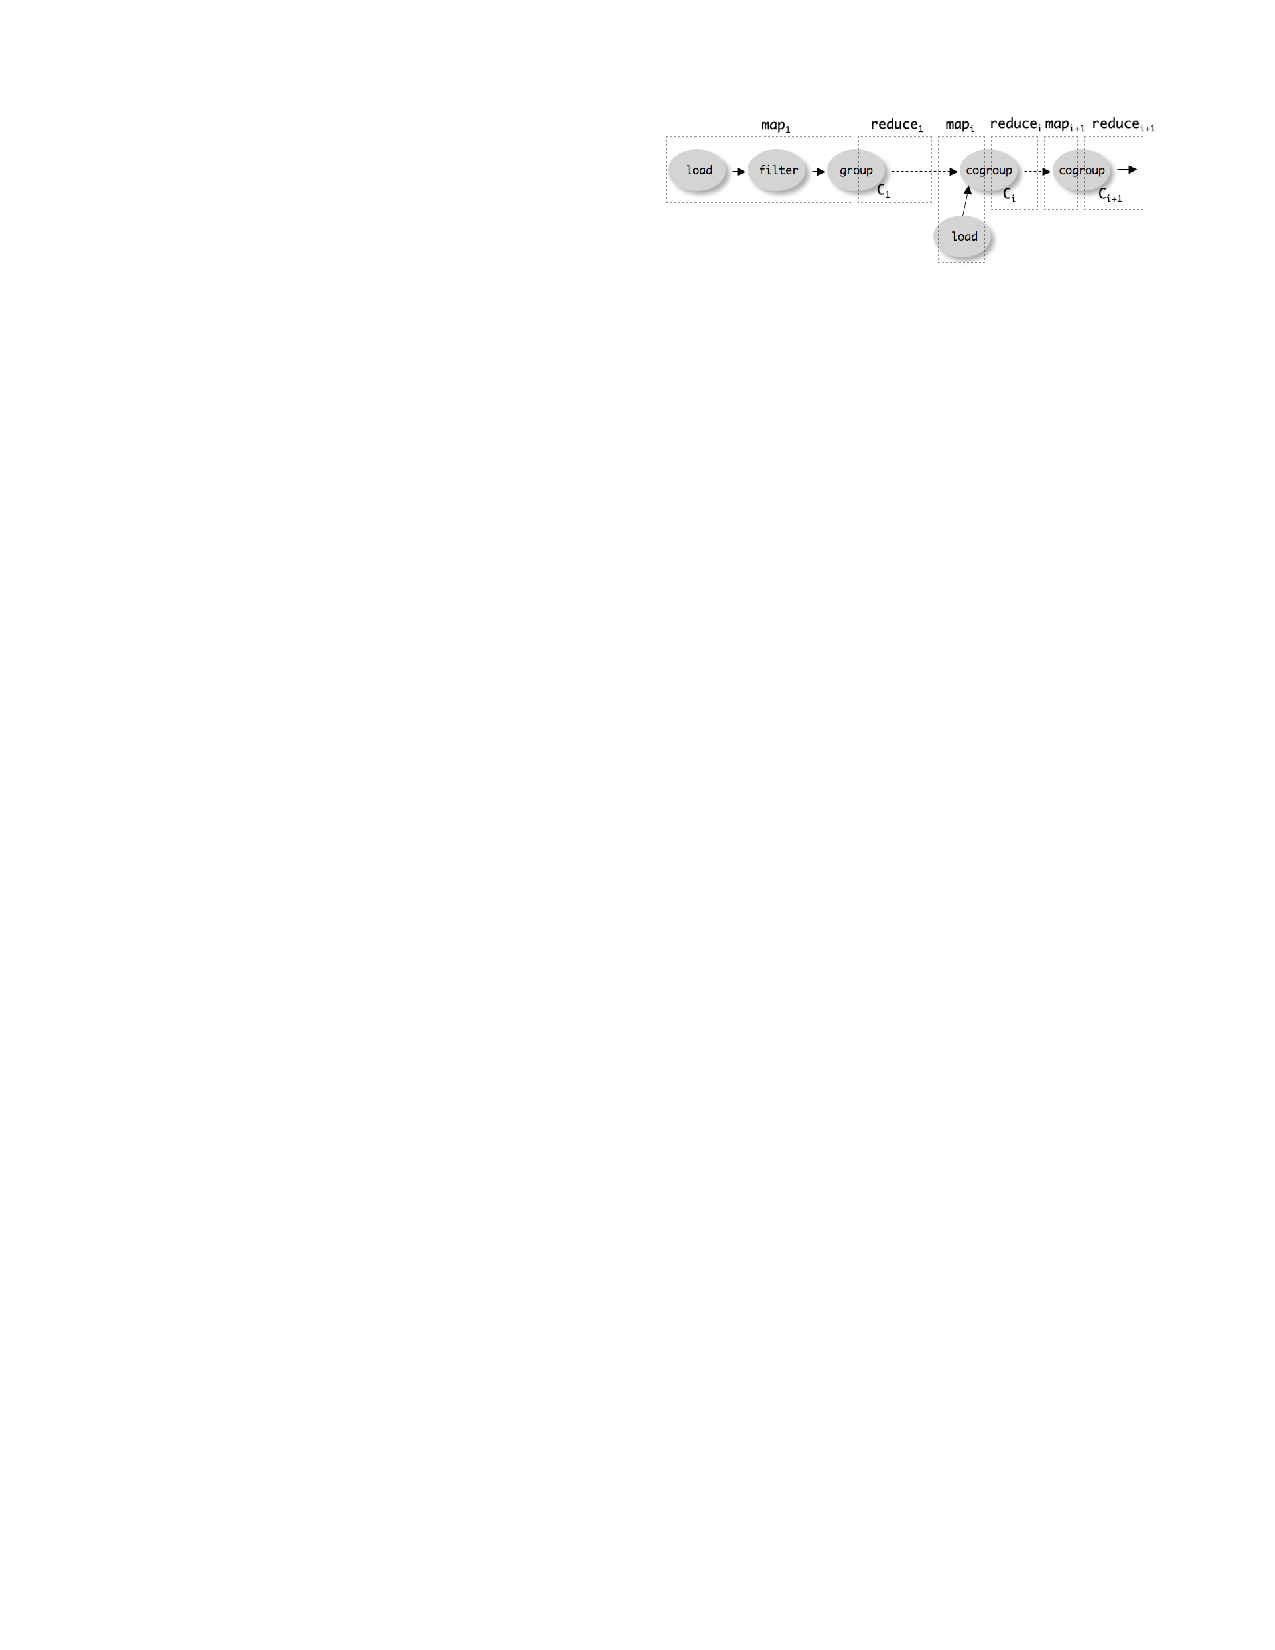
\includegraphics[scale=1.2]{./Figures/compiler}
  \end{figure}

  \begin{itemize}
  \item \textbf{MapReduce boundary is the \texttt{COGROUP} command} 
    \begin{itemize}
    \item The sequence of \texttt{FILTER} and \texttt{FOREACH} from
      the \texttt{LOAD} to the first \texttt{COGROUP} $C_1$ are pushed
      in the Map function
    \item The commands in later \texttt{COGROUP} commands $C_i$ and
      $C_{i+1}$ can be pushed into:
      \begin{itemize}
      \item the Reduce function of $C_i$
      \item the Map function of $C_{i+1}$
      \end{itemize}
    \end{itemize}
  \end{itemize}
}

%%%%%%%%%%%%%%%%%%%%%%%%%%%%%%%%%%%%%%%%%%%%%%%%%%%%%%%%%%
\frame {\frametitle{Building the Physical Plan}
%%%%%%%%%%%%%%%%%%%%%%%%%%%%%%%%%%%%%%%%%%%%%%%%%%%%%%%%%%
  \begin{itemize}
  \item \textbf{Pig optimization for the physical plan}
    \begin{itemize}
    \item Among the two options outlined above, the first is preferred
    \item Indeed, grouping is often followed by aggregation
    \item[$\to$] {\color{red}reduces the amount of data to be
        materialized between jobs}
    \end{itemize}

    \vspace{20pt}

  \item \textbf{\texttt{COGROUP} command with more than one input dataset}
    \begin{itemize}
    \item Map function appends an extra field to each tuple to
      identify the dataset
    \item Reduce function decodes this information and inserts tuple
      in the appropriate nested bags for each group
    \end{itemize}

  \end{itemize}
}

%%%%%%%%%%%%%%%%%%%%%%%%%%%%%%%%%%%%%%%%%%%%%%%%%%%%%%%%%%
\frame {\frametitle{Building the Physical Plan}
%%%%%%%%%%%%%%%%%%%%%%%%%%%%%%%%%%%%%%%%%%%%%%%%%%%%%%%%%%
  \begin{itemize}
  \item \textbf{How parallelism is achieved}
    \begin{itemize}
    \item For \texttt{LOAD} this is inherited by operating over HDFS
    \item For \texttt{FILTER} and \texttt{FOREACH}, this is automatic
      thanks to MapReduce framework
    \item For \texttt{(CO)GROUP} uses the \texttt{SHUFFLE} phase
    \end{itemize}

    \vspace{20pt}

  \item \textbf{A note on the \texttt{ORDER} command}
    \begin{itemize}
    \item Translated in two MapReduce jobs
    \item First job: {\color{red}Samples the input} to determine quantiles of the
      sort key
    \item Second job: Range partitions the input according to
      quantiles, followed by sorting in the reduce phase
    \end{itemize}

    \vspace{20pt}

  \item \textbf{Known overheads due to MapReduce inflexibility}
    \begin{itemize}
    \item Data materialization between jobs
    \item Multiple inputs are not supported well
    \end{itemize}

  \end{itemize}
}

%%%%%%%%%%%%%%%%%%%%%%%%%%%%%%%%%%%%%%%%%%%%%%%%%%%%%%%%%%
\frame {\frametitle{Summary}
%%%%%%%%%%%%%%%%%%%%%%%%%%%%%%%%%%%%%%%%%%%%%%%%%%%%%%%%%%
  \begin{figure}[h]
    \centering
    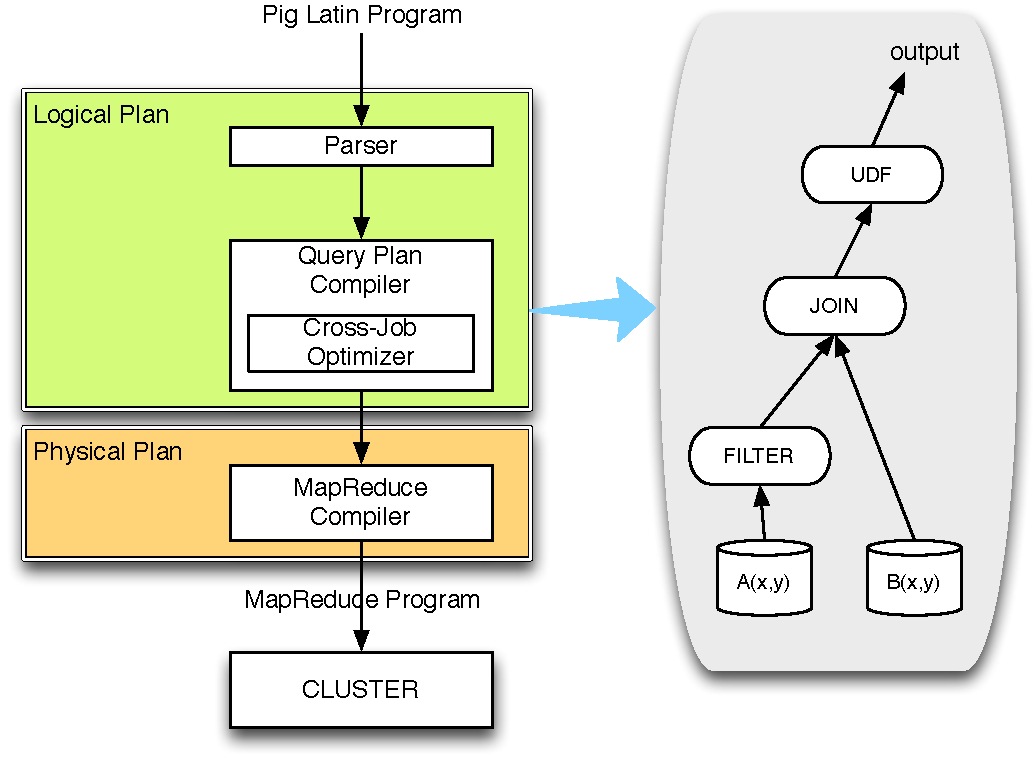
\includegraphics[scale=0.5]{./Figures/pig_overview}
  \end{figure}
}

%%%%%%%%%%%%%%%%%%%%%%%%%%%%%%%%%%%%%%%%%%%%%%%%%%%%%%%%%%
\frame {\frametitle{Single-program Optimizations}
%%%%%%%%%%%%%%%%%%%%%%%%%%%%%%%%%%%%%%%%%%%%%%%%%%%%%%%%%%
  \begin{itemize}
  \item \textbf{Logical optimizations: query plan}
    \begin{itemize}
    \item Early projection
    \item Early filtering
    \item Operator rewrites
    \end{itemize}

    \vspace{20pt}

  \item \textbf{Physical optimization: execution plan}
    \begin{itemize}
    \item Mapping of logical operations to MapReduce
    \item Splitting logical operations in multiple physical ones
    \item Join execution strategies
    \end{itemize}
  \end{itemize}
}

%%%%%%%%%%%%%%%%%%%%%%%%%%%%%%%%%%%%%%%%%%%%%%%%%%%%%%%%%%
\frame {\frametitle{Efficiency measures}
%%%%%%%%%%%%%%%%%%%%%%%%%%%%%%%%%%%%%%%%%%%%%%%%%%%%%%%%%%
  \begin{itemize}
  \item \textbf{\texttt{(CO)GROUP} command places tuples of the same group in
      nested bags}
    \begin{itemize}
    \item Bag materialization (I/O) can be avoided
    \item This is important also due to memory constraints
    \item {\color{red}Distributive} or {\color{red}algebraic}
      aggregation facilitate this task
    \end{itemize}

    \vspace{20pt}

  \item \textbf{What is an algebraic function?}
    \begin{itemize}
    \item Function that can be structured as a tree of sub-functions
    \item Each leaf sub-function operates over a subset of the input
      data
    \item[$\to$] If nodes in the tree achieve data reduction, then the system
      can reduce materialization
    \item Examples: \texttt{COUNT}, \texttt{SUM}, \texttt{MIN},
      \texttt{MAX}, \texttt{AVERAGE}, ...
    \end{itemize}

  \end{itemize}
}

%%%%%%%%%%%%%%%%%%%%%%%%%%%%%%%%%%%%%%%%%%%%%%%%%%%%%%%%%%
\frame {\frametitle{Efficiency measures}
%%%%%%%%%%%%%%%%%%%%%%%%%%%%%%%%%%%%%%%%%%%%%%%%%%%%%%%%%%
  \begin{itemize}
  \item \textbf{Pig compiler uses the {\color{red}combiner} function
      of Hadoop}
    \begin{itemize}
    \item A special API for algebraic UDF is available
    \end{itemize}

    \vspace{20pt}

  \item \textbf{There are cases in which \texttt{(CO)GROUP} is
      inefficient}
    \begin{itemize}
    \item This happens with non-algebraic functions
    \item Nested bags can be spilled to disk
    \item Pig provides a {\color{red}disk-resident bag implementation}
      \begin{itemize}
      \item Features external sort algorithms
      \item Features duplicates elimination
      \end{itemize}
    \end{itemize}
  \end{itemize}
}
